
\documentclass[a4paper,fleqn]{cas-dc}
\usepackage[authoryear,longnamesfirst]{natbib}

\usepackage{nicefrac}
\usepackage{amsthm}
\usepackage{ragged2e}
\usepackage{dsfont}

\numberwithin{equation}{section}
\newcommand{\R}{\mathds{R}}
\newcommand{\N}{\mathds{N}}
\newcommand{\Nzero}{\mathds{N}_0}
\newcommand{\Pp}{\mathds{P}}
\newcommand{\E}{\mathds{E}}
\newcommand{\1}{\mathds{1}}
\newcommand{\dd}{\mathrm{d}}
\newcommand{\norm}[1]{\left\lVert #1\right\rVert}
\newcommand{\set}[1]{\left\{#1\right\}}
\newcommand{\Leb}{\lambda}
\newcommand{\ellpq}{\ell_{p,q}}
\newcommand{\ellox}{\ell_{\mathbf{0},x}}
\newcommand{\upq}{u_{p,q}}
\newcommand{\0}{\mathbf{0}}

\DeclareMathOperator{\Exp}{Exp}
\DeclareMathOperator{\Po}{Po}
\DeclareMathOperator{\diam}{diam}
\newtheorem{theorem}{Theorem}[section]
\newtheorem{corollary}[theorem]{Corollary}
\newtheorem{proposition}[theorem]{Proposition}
\newtheorem{lemma}[theorem]{Lemma}
\newtheorem{definition}[theorem]{Definition}
\newtheorem{example}[theorem]{Example}

\emergencystretch=1em

\begin{document}
\let\WriteBookmarks\relax
\def\floatpagepagefraction{1}
\def\textpagefraction{.001}

\shorttitle{Unit-region factorization for empty-region proximity graphs}
\shortauthors{H. Espino-Montelongo and H. Maravillo}

\title[mode=title]{Unit-Region Factorization for Empty-Region Proximity Graphs}

\author[1]{Heriberto {Espino-Montelongo}}[
  orcid=0009-0009-1230-2931
]
\cormark[1]
\ead{heriberto.espinomo@udlap.mx}
\credit{Conceptualization, Methodology, Formal analysis, Investigation, Validation, Visualization, Writing -- original draft}

\author[2]{H\'ector {Maravillo}}[
  orcid=0000-0002-6101-1964
]
\ead{hector.maravillo@uacm.edu.mx}
\credit{Conceptualization, Investigation, Supervision, Writing -- review and editing}

\affiliation[1]{
  organization={Universidad de las Am\'ericas Puebla},
  addressline={Ex Hacienda Santa Catarina M\'artir S/N},
  city={San Andr\'es Cholula},
  postcode={72810},
  state={Puebla},
  country={Mexico}
}

\affiliation[2]{
  organization={Universidad Aut\'onoma de la Ciudad de M\'exico},
  addressline={Dr. Garc\'ia Diego 168, Col. Doctores,
               Alcald\'ia Cuauht\'emoc},
  city={Ciudad de M\'exico},
  postcode={06720},
  country={Mexico}
}

\cortext[cor1]{Corresponding author.}

\begin{abstract}
Many proximity graphs join two sites when a region determined by the pair contains no other site. We study finite empty-region rules for which the region associated with each pair is obtained from a fixed normalized Borel region by translation, rotation, and uniform scaling. If \(a_K\) denotes the volume of the unit region, then the corresponding pairwise region has volume \(a_K\ellpq^d\), where \(d\) is the dimension and \(\ellpq\) is the pair length. Thus, at the first-order stochastic level, the geometry of the rule enters through the single scalar \(a_K\).

For a homogeneous Poisson process, this factorization yields the exact
fixed-pair void probability and, for any Borel unit-region rule, the
incident-edge length intensity, mean out-degree, and normalized
incident-edge length law. For symmetric rules, the out-degree coincides
with the ordinary degree. The normalized incident-edge length law is
Weibull with shape parameter \(d\) and scale
\((\rho a_K)^{-\nicefrac{1}{d}}\).
Explicit formulas for the \(d\)-dimensional volume \(a_K\) are given
for several proximity graphs, including the Gabriel graph, the relative-neighborhood graph,
lune-based \(\beta\)-skeletons, and stepping--stone graphs. In the
planar case, the framework also covers the circle-based
\(\beta\)-skeleton through Veltkamp's diagonal parameterization,
together with selected prescribed two-ball regions associated with
Veltkamp's \(\gamma\)-neighborhood construction.




\end{abstract}


\begin{keywords}
Empty-region graph \sep proximity graph \sep Poisson point process \sep Palm distribution \sep computational geometry \sep stochastic geometry
\end{keywords}

\maketitle

\hypersetup{
  pdftitle={Unit-Region Factorization for Empty-Region Proximity Graphs},
  pdfauthor={Heriberto Espino-Montelongo and H\'ector Maravillo},
  pdfsubject={Unit-region factorization for empty-region proximity graphs},
  pdfkeywords={empty-region graph, proximity graph, Poisson point process, Palm distribution, computational geometry, stochastic geometry}
}

\section{Introduction}

Proximity graphs are graphs defined on point sets in Euclidean space, in which two points are adjacent whenever they are sufficiently close according to some geometric criterion. A major subclass is based on empty-region rules: a region is associated with a candidate pair of points, and the pair is adjacent whenever this region contains no other points of the set \citep{jaromczyk1992relative,cardinal2009empty}. Originally, motivated by their main applications, proximity graphs were defined for point sets in the plane, but their definition naturally extends to higher-dimensional spaces \citep{jaromczyk1991constructing,devroye1988expected}. Classical examples include the Gabriel graph, the relative neighborhood graph, the nearest neighbor graphs, $\beta$-skeletons, and the sphere-of-influence graph \citep{jaromczyk1992relative,mitchell2018,mathieson2019}. Proximity graphs have been used in geographic analysis \citep{gabriel1969statistical}, data mining \citep{toussaint2005geometric}, topological data analysis \citep{correa2011towards,jurkiewicz2023topohub}, machine learning \citep{marchette2005random,toussaint2012proximity}, modeling urban street networks \citep{watanabe2008evaluating,maravillo2023recovering}, communication and wireless-network design \citep{iguchi2008localized}, and even in archaeological studies \citep{jimenez2002application}. For further applications, see \citep{jaromczyk1992relative,toussaint2014applications,toussaint2014sphere}.

Proximity graphs have been extensively studied from both algorithmic and theoretical perspectives \citep{cimikowski1990coloring,hurtado2003optimal,cardinal2009empty,bose2012proximity,kowaluk2015new}. Their probabilistic properties have also received considerable attention for graphs built on random point sets. \citet{devroye1988expected} determined the expected size of empty-region graphs on $n$ i.i.d. points with an arbitrary density in $\mathds{R}^d$ under suitable regularity and symmetry assumptions on the associated regions. \citet{alonso2019geometrical} computationally analyzed the average degree of $\beta$-skeletons constructed on points uniformly distributed in the planar unit square. \citet{watanabe2008evaluating} derived the expected length of the edges of the relative neighborhood graph of a planar homogeneous Poisson process in terms of its intensity. More recently, \citet{sambale2026limit} established limit laws for longest edges in several empty-region graphs generated by stationary Poisson point processes.

The present paper continues this line of research on the probabilistic properties of proximity graphs. We consider empty-region graphs generated by a homogeneous Poisson point process in $\mathds{R}^d$, allowing arbitrary defining regions that are Borel sets with finite positive Lebesgue measure. This framework includes well-known examples such as the Gabriel graph, the relative neighborhood graph, and $\beta$-skeletons. Our main contributions are summarized below:

\paragraph{Geometric factorization.}
The paper identifies a class of finite similarity-region empty-region rules and proves that the region $S(p,q)$ associated with each pair $p \neq q$ has volume
\begin{equation}
\lambda_d\bigl(S(p,q)\bigr) = a_K\|p-q \|^d,
\end{equation}
where $\lambda_d$ is the $d$-dimensional Lebesgue measure and $a_K$
is the volume of the unit region. Thus the geometric dependence of every rule in the class is reduced to one region-volume constant. 

\paragraph{Poisson--Palm consequences.}
For a homogeneous Poisson process with intensity \(\rho\), the
factorization yields the exact fixed-pair void probability, the mean
out-degree, and the normalized incident-edge length law. For symmetric
rules, the out-degree is the ordinary degree. The normalized
incident-edge length law is Weibull with shape parameter \(d\) and
scale parameter \((\rho a_K)^{-\nicefrac{1}{d}}\).


\paragraph{Explicit ball-generated constants.}
\leavevmode\\
Using hyperspherical-cap formulas, the paper derives explicit
\(d\)-dimensional volume constants for lune-based \(\beta\)-skeleton
regions. In the planar case, the same cap formulas apply to the
diagonal Veltkamp subfamily, which recovers the circle-based
\(\beta\)-skeleton, and to selected prescribed two-ball regions
associated with Veltkamp's \(\gamma\)-neighborhood construction.


 \paragraph{Stepping-stone volume constant.}
For the stepping--stone diversion region, the paper derives a dimension-uniform integral representation for the volume of the unit region.
This makes the unit-region factorization explicit for the stepping--stone family and therefore yields its Poisson--Palm consequences.\\

The remainder of the paper is organized as follows.
Section \ref{sec:notation} establishes the notation and standing assumptions.
Section \ref{sec:unit-region} introduces the similarity-region framework and proves the unit-region volume factorization.
Section \ref{sec:poisson} derives its consequences for homogeneous Poisson input, including the fixed-pair void probability and the Palm incident-edge results.
Section \ref{sec:examples} evaluates the region-volume constants for the principal examples.
Section \ref{sec:discussion} discusses the scope, limitations, and possible extensions of the framework.
Section \ref{sec:conclusion} concludes.



\section{Notation and standing conventions}\label{sec:notation}

Throughout the paper, we work in the Euclidean space \(\R^d\), with ambient dimension \(d\geq2\), equipped with the Euclidean norm \(\norm{\cdot}\) and the $d$-dimensional Lebesgue measure \(\lambda_d\). We write $\0$ for the origin  and \(e_1=(1,0,\ldots,0)\) for the first coordinate vector. 

For \(x\in\R^d\) and \(r\ge0\), let
\begin{equation}
        B(x,r):=\set{y\in\R^d:\norm{y-x}\le r}
\end{equation}
be the closed Euclidean ball.  Its volume is
\begin{equation}\label{eq:ball-volume}
        \lambda_d(B(x,r))=\kappa_d r^d,
\end{equation}
where
\begin{equation}
        \kappa_d:=\lambda_d(B(\0,1))
        =
        \frac{\pi^{\nicefrac{d}{2}}}{\Gamma\left(1+\nicefrac{d}{2}\right)},
\end{equation}
and \(\Gamma\) is Euler's gamma function.

For every candidate pair \(p\neq q\in \R^d\), define
\begin{equation}\label{eq:ell-direction}
        \ellpq:=\norm{p-q},
        \qquad
        \upq:=\frac{q-p}{\ellpq}.
\end{equation}
Thus \(\ellpq\) is the pair length and \(\upq\) is the unit vector 
from \(p\) to \(q\).  When a rotation is needed, \(R_{p,q}\in O(d)\) denotes
an orthogonal map satisfying
\(
        R_{p,q}e_1=\upq .
\)
The affine map 
\begin{equation}
        T_{p,q}(z):=p+\ellpq R_{p,q}z
\end{equation}
 sends the normalized segment \([\0,e_1]\) to \([p,q]\).  

The symbol \(K\subset\R^d\) denotes a normalized unit region, and
\begin{equation}
    a_K:=\lambda_d(K)
\end{equation}
denotes its unit volume. 

Let \(V\subset \R^d\) be a finite or locally finite set of points. To each pair of distinct points $p,q\in V$, associate a region or neighborhood $S(p,q)\subset \R^d$. A neighborhood graph, also called proximity graph, is a graph  $G=(V,E)$ whose edge set is determined by a property $\mathrm{p}$ of these regions: namely, $(p,q)\in E$ if and only if $S(p,q)$ satisfies $\mathcal{P}$ \citep{jaromczyk1992relative}. When the property $\mathcal{P}$ consists of the empty-region rule
\begin{equation}
    S(p,q)\cap (V\setminus\{p,q\})=\emptyset.
\end{equation}
For a nonsymmetric rule, this condition defines a directed arc
\(p\to q\). When the rule is symmetric, this condition also holds with
\(p\) and \(q\) interchanged and defines the undirected edge
\(\{p,q\}\).
The resulting graph is known as an empty-region graph, and the pair \(p, q\) that satisfy this criterion are called adjacent; see \citet{cardinal2009empty}. The choice of the regions $S(p,q)$ determines several well-known proximity graphs, such as nearest-neighbor graphs, the Gabriel graph \citep{gabriel1969statistical}, the relative-neighborhood graph \citep{toussaint1980relative}, $\beta$-skeletons \citep{kirkpatrick1985framework}, $\gamma$-neighborhood graphs \citep{veltkamp1992gamma}, and stepping--stone graphs \citep{kannangara2018stepping}.

In this paper, we restrict attention to  Borel sets \(S(p,q)\) satisfying  \(0<\lambda_d(S(p,q))<\infty  \). 

In the probabilistic sections, \(\Phi\) denotes a homogeneous Poisson point
process on \(\R^d\) with intensity measure \(\rho\lambda_d\), where
\(\rho>0\).  The symbols \(\Pp\) and \(\E\) denote probability and expectation. For \(z\in\R^d\), let \(\Pp^z\) denote the Palm probability of \(\Phi\) at \(z\), and let \(\E^z\) denote the corresponding expectation. In particular, Palm probability and expectation at the origin are denoted by \(\Pp^{\0}\) and
\(\E^{\0}\), respectively.


The set \(
        \Nzero:=\{0,1,2,\ldots\}
\)
is used for order-\(k\) empty-region rules. 
Boundary conventions are fixed in
the deterministic graph definition: the empty region may be open, closed, or
given by an interior. 
Here \(\partial S(p,q)\) denotes the boundary of the pair region \(S(p,q)\).
For Poisson point process whose intensity measure is absolutely
continuous with respect to \(\lambda_d\), these conventions give the same void probabilities whenever
\(
     \lambda_d(\partial S(p,q))=0.   
\)
For deterministic point sets, the chosen boundary convention can change the
edge set when data points lie on \(\partial S(p,q)\).


\section{Unit regions}\label{sec:unit-region}

\begin{definition}[Unit region]\label{def:unit-region}
Assume that \(S\) is a measurable translation-covariant pairwise empty-region rule. Then \(S\) has a unit region if there is a Borel set $K\subset\R^d$ with $0<\lambda_d(K)<\infty$ such that, for every $p\neq q \in \R^d$, there exists $R_{p,q}\in O(d)$ satisfying
\begin{eqnarray}
    R_{p,q}e_1 &=& \upq\\
    S(p,q) &=& p+\ellpq R_{p,q}K.\label{eq:unit-region}
\end{eqnarray}
\end{definition}

The same condition can be expressed as a unit-region construction with a fixed normalized region that is translated, rotated, and uniformly scaled according to the candidate pair \citep{cardinal2009empty}. It is also implied by set-level similarity equivariance.


\begin{figure*}[width=\textwidth,pos=ht]
\centering
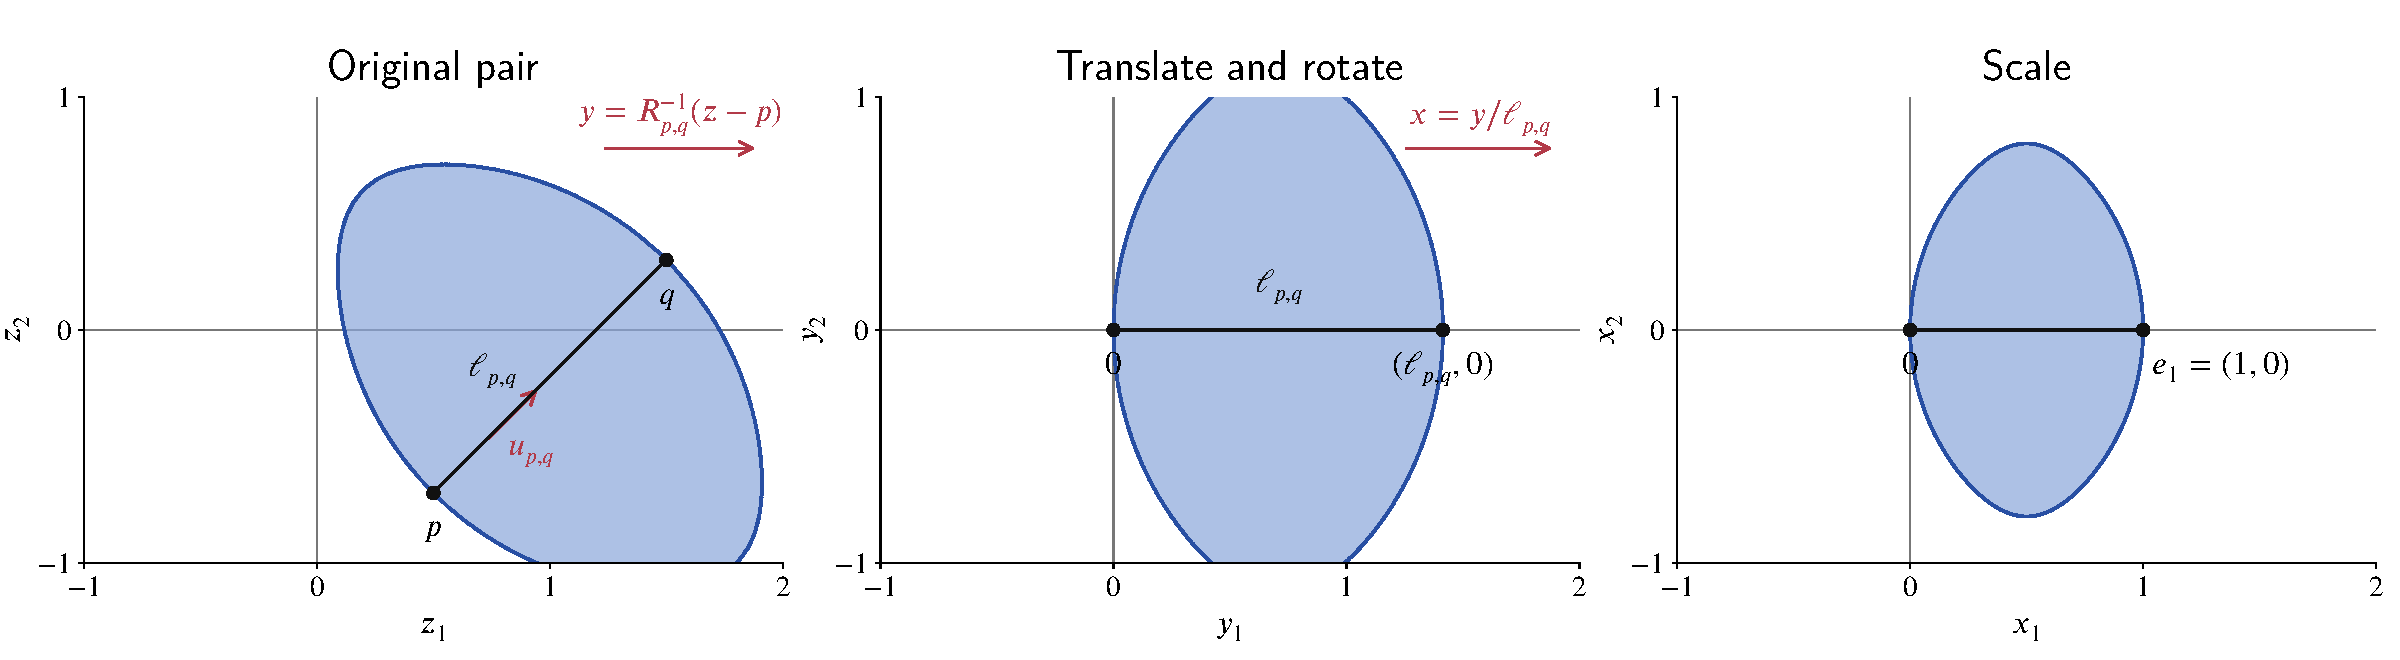
\includegraphics[width=\textwidth]{normalization_map_ell.pdf}
\caption{Normalization of a pairwise empty region. Starting from a
candidate pair \(p,q\), translate by \(-p\), rotate the segment
\(q-p\) onto the \(e_1\)-axis, and scale by \(\ell_{p,q}^{-1}\).
The resulting normalized region is the unit region \(K\), while the
original pair region is recovered as
\(S(p,q)=p+\ell_{p,q}R_{p,q}K\).}
\label{fig:normalization-map}
\end{figure*}

\begin{proposition}[Similarity equivariance gives a unit region]\label{prop:equivariance-unit}
Suppose that \(S\) is measurable and that, for every Euclidean
similarity \(T(x)=\tau Rx+a\), with \(\tau>0\), \(R\in O(d)\), and
\(a\in\mathbb R^d\), one has
\begin{equation}
        S\left(T(p),T(q)\right)=T\left(S(p,q)\right).
\end{equation}
Then $S$ has a unit region, namely $K=S(\0,e_1)$.
\end{proposition}

\begin{proof}
For $p\neq q$, choose $R_{p,q}\in O(d)$ with $R_{p,q}e_1=\upq$.  The similarity $T(x)=p+\ellpq R_{p,q}x$ maps $[\0,e_1]$ to $[p,q]$.
Hence
\begin{equation}
\begin{aligned}
S(p,q)
&=S\left(T(\0),T(e_1)\right)\\
&=T\left(S(\0,e_1)\right)
 =p+\ellpq R_{p,q}K.
\end{aligned}
\end{equation}
Thus, similarity equivariance yields the required unit-region representation.
\end{proof}

For $d\geq 3$, many orthogonal maps send $e_1$ to $\upq$.  The volume identity is independent of this choice, since every orthogonal map preserves $\lambda_d$.  The graph-level definition also needs a definite orientation convention when $K$ lacks axial symmetry around the $e_1$-axis.  This can be supplied by a measurable choice $(p,q)\mapsto R_{p,q}$, or by imposing invariance of $K$ under all rotations fixing $e_1$. The regions associated with the Gabriel graph, the relative-neighborhood graph, $\beta$-skeletons, and stepping--stone graphs satisfy this axial-symmetry condition.

\begin{theorem}[Unit-region factorization]\label{thm:factorization}
If $S$ has a unit region $K$, then for $p\neq q\in \R^d$
\begin{equation}\label{eq:factorization}
        \lambda_d(S(p,q))=a_K\ellpq^d.
\end{equation}
\end{theorem}

\begin{proof}
Translation and orthogonal maps preserve Lebesgue measure. Scaling by $\ellpq$ multiplies $d$-dimensional volume by $\ellpq^d$. Applying this to \eqref{eq:unit-region} gives
\begin{equation}
        \lambda_d(S(p,q))
        =\lambda_d\bigl(p+\ellpq R_{p,q}K\bigr)
        =\ellpq^d\lambda_d(K).
\end{equation}
Therefore, the volume of the pair region factors into the unit-region
constant and the distance scale.
\end{proof}






\section{Poisson void probabilities and Palm consequences}\label{sec:poisson}


A pairwise empty-region rule is a geometric
construction. Given a locally finite configuration
\(\eta\subset\R^d\), two distinct points \(p,q\in\eta\) are adjacent
when the region \(S(p,q)\) associated with the pair contains no point
of \(\eta\) other than the endpoints. Thus, the empty-region condition
is
\begin{equation}
\eta\bigl(S(p,q)\setminus\{p,q\}\bigr)=0,
\end{equation}
where \(\eta(A)\) denotes the
number of points of \(\eta\) contained in a Borel set \(A\subseteq\R^d\).

In this section, the vertex configuration is a homogeneous Poisson
point process. The deterministic empty-region condition then becomes a
Poisson void event. The unit-region factorization established in
Section~\ref{sec:unit-region} implies that the volume of the region
associated with a pair depends only on its length and on the region
constant:
\begin{equation}\label{eq:section-factorization}
\begin{aligned}
\lambda_d\bigl(S(p,q)\setminus\{p,q\}\bigr)
&=\lambda_d\bigl(S(p,q)\bigr)\\
&=a_K\ellpq^d,\qquad p\neq q.
\end{aligned}
\end{equation}
Hence, for the homogeneous Poisson model, the geometric effect of the
rule enters the fixed-pair calculation through the single scalar
\(a_K\).

Let \(\Phi\) be a homogeneous Poisson point process on \(\R^d\) with
intensity measure \(\rho\lambda_d\), where \(\rho>0\). For every Borel
set \(A\subset\R^d\) with \(\lambda_d(A)<\infty\),
\begin{equation}\label{eq:poisson}
\Phi(A)
\sim
\operatorname{Poisson}\bigl(\rho\lambda_d(A)\bigr),
\end{equation}
and the counts on disjoint Borel sets are independent. In particular,
\begin{equation}\label{eq:void}
\Pp\left\{\Phi(A)=0\right\}
=
\exp\left\{-\rho\lambda_d(A)\right\}.
\end{equation}
Equation~\eqref{eq:void} is the Poisson void probability; see
\citep{last2017lectures,baccelli2010stochastic}.



\begin{corollary}[Fixed-pair Poisson void law]
\label{cor:fixed-pair}
For every deterministic pair \(p\neq q\),
\begin{equation}\label{eq:fixed-pairr}
\Pp\left\{\Phi\bigl(S(p,q) \setminus \{p,q\}\bigr)=0\right\}
=
\exp\left\{
-\rho a_K \ellpq^{d}
\right\}.
\end{equation}
Equivalently, \eqref{eq:fixed-pairr} is the probability that the
prescribed pair \(p,q\) is adjacent after the two points are inserted
into an independent Poisson configuration.
\end{corollary}

Corollary~\ref{cor:fixed-pair} concerns a prescribed candidate pair. We now pass to the local neighborhood of a typical point of the process. Let $\Pp^{\0}$ denote the Palm distribution of $\Phi_\0$ at the origin, and let $\Phi_{\0}^{!}$ be the associated reduced Palm process. Under $\Pp^{\0}$, the configuration may be viewed as a distinguished point at $\0$ together with the remaining process $\Phi_{\0}^{!}$; hence the candidate neighbors are the points of $\Phi_{\0}^{!}$. By the Mecke--Slivnyak theorem,
\begin{equation}\label{eq:reduced-palm-poisson}
\Phi_{\0}^{!} \overset{d}{=} \Phi,
\end{equation}
where the process on the right is again a homogeneous Poisson process with intensity measure $\rho\lambda_d$; see \citep{baccelli2010stochastic,last2017lectures}.


\begin{corollary}[Typical points Poisson void law]
\label{cor:typical-pair}
For every two typical points \((p,q)\) with \(p\neq q\),
\begin{equation}\label{eq:two-point-palm-acceptance}
\Pp^{p,q}\left\{
\Phi^{!}_{p,q}\bigl(S(p,q)\bigr)=0
\right\}
=
\exp\left\{
-\rho a_K \ellpq^{d}
\right\}.
\end{equation}
\end{corollary}

\begin{proof}
The two-point Palm identity follows
from Slivnyak's theorem, since \(\Phi^{!}_{p,q}\) has the same
distribution as \(\Phi\).
Apply the Poisson void formula \eqref{eq:void} to \(S(p,q)\), then use
\(\lambda_d(S(p,q))=a_K\ellpq^d\). 
\end{proof}

For a candidate point \(x\in\eta\), define
\begin{equation}
\label{eq:palm-edge-indicator}
\chi_K(x;\eta)
:=
\1\!\left\{
\eta\!\left(
S(\0,x)\setminus\{\0,x\}
\right)=0
\right\}.
\end{equation}
Thus \(\chi_K(x;\eta)=1\) precisely when no point of \(\eta\)
other than the endpoints \(\0\) and \(x\) lies in the pair
region \(S(\0,x)\). In particular, under the reduced Palm
distribution,
\begin{equation}
\chi_K(x;\Phi_{\0}^{!})=1
\end{equation}
if and only if the directed edge that goes from the Palm point to \(x\) is present. If the rule is symmetric, namely
\begin{equation}
S(p,q)=S(q,p),
\qquad p\neq q,
\end{equation}
then this is equivalent to the undirected edge
\(\{\0,x\}\) being incident to the Palm point.


\begin{corollary}[Palm--Mecke identity for incident edges]
\label{cor:palm-mecke}
For every nonnegative measurable function
\(g\colon\R^d\to[0,\infty)\),
\begin{equation}\label{eq:palm-mecke-acceptance}
\begin{aligned}
\E^{\0}\left[
\sum_{x\in\Phi_\0^!} g(x)\chi_K(x;\Phi_\0^!)
\right]
&=\rho\int_{\R^d}g(x)\\
&\quad{}\times\exp\left\{-\rho a_K\ellox^{d}\right\}\,\dd x.
\end{aligned}
\end{equation}
\end{corollary}

\begin{proof}
By \eqref{eq:reduced-palm-poisson}, the reduced Palm process
\(\Phi_\0^!\) has the same distribution as a homogeneous Poisson process of
intensity \(\rho\lambda_d\). Applying the Mecke formula to \(\Phi_\0^!\)
therefore yields
\begin{equation}
\begin{aligned}
\E^{\0}\left[
\sum_{x\in\Phi_\0^!} g(x)\chi_K(x;\Phi_\0^!)
\right]
&=\rho\int_{\R^d}g(x)\\
&\quad{}\times\Pp\left\{\Phi\bigl(S(\0,x)\bigr)=0\right\}\,\dd x.
\end{aligned}
\end{equation}
By Corollary~\ref{cor:fixed-pair},
\begin{equation}
\Pp\left\{
\Phi\bigl(S(\0,x)\bigr)=0
\right\}
=
\exp\left\{-\rho a_K\ellox^{d}\right\}.
\end{equation}
Substitution gives \eqref{eq:palm-mecke-acceptance}.
\end{proof}

The deterministic integration variable $x$ in \eqref{eq:palm-mecke-acceptance} represents the displacement of a candidate neighbor from the Palm point. Although the exclusion region $S(\0,x)$ may depend on the direction of $x$ through the rotated region $K$, unit-region factorization depends on the candidate displacement only through $\ellox$ and on the region only through its volume constant $a_K = \lambda_d(K)$. Thus, at this first-order void-probability level, the detailed shape of $K$ does not enter beyond its volume.


\begin{definition}[Palm incident-edge length measure]
\label{def:palm-length-measure}
Define a measure \(\nu_K\) on \([0,\infty)\) by
\begin{equation}\label{eq:palm-length-measure-eq}
\nu_K(C)
:=
\E^{\0}\left[
\sum_{x\in\Phi_\0^!}
\chi_K(x;\Phi_{\0}^!)
\1\left\{\ellox\in C\right\}
\right],
\end{equation}
for every Borel set \(C\subset[0,\infty)\).

Thus \(\nu_K(C)\) is the expected number of edges from the Palm point whose Euclidean lengths belong to \(C\). In general, \(\nu_K\) is a finite
first-moment measure.
In the nonsymmetric setting, this measure concerns edges directed
outward from the Palm point. Under symmetry, these are the usual
undirected edges incident to that point.
\end{definition}

\begin{corollary}[Incident-edge length law]
\label{cor:palm-intensity}
The Palm incident-edge length measure \(\nu_K\) is absolutely continuous with
respect to Lebesgue measure and satisfies
\begin{equation}\label{eq:palm-intensity}
\nu_K(\dd r)
=
\rho d\kappa_d r^{d-1}
\exp\left\{-\rho a_Kr^d\right\}
\,\dd r,
\qquad r\geq0.
\end{equation}
Equivalently, for every \(r\geq0\),
\begin{equation}\label{eq:incident-edge-cdf-measure}
\nu_K([0,r])
=
\frac{\kappa_d}{a_K}
\left(
1-\exp\left\{-\rho a_Kr^d\right\}
\right).
\end{equation}
\end{corollary}

\begin{proof}
Let \(h\colon[0,\infty)\to[0,\infty)\) be measurable. By
Definition~\ref{def:palm-length-measure} and
Corollary~\ref{cor:palm-mecke}, applied with \(g(x)=h(\ellox)\),
\begin{equation}
\begin{aligned}
\int_{[0,\infty)}
h(r)\,\nu_K(\dd r)
&=
\rho\int_{\R^d}h(\ellox)\\
&\quad{}\times\exp\left\{-\rho a_K\ellox^{d}\right\}\,\dd x.
\end{aligned}
\end{equation}

The integrand is radial because it is a function only of
\(\ellox=\|x\|\); equivalently, it is invariant under every
orthogonal transformation \(Q\in O(d)\), since
\(
\|Qx\|=\|x\|.
\)
Hence polar coordinates in \(\R^d\), with \(d\kappa_d\) equal to the
surface area of the unit sphere in \(\R^d\), yield
\begin{equation}
\begin{aligned}
\int_{[0,\infty)}
h(r)\,\nu_K(\dd r)
&=
\rho d\kappa_d\int_0^\infty h(r)r^{d-1}\\
&\quad{}\times\exp\left\{-\rho a_Kr^d\right\}\,\dd r.
\end{aligned}
\end{equation}
Since this holds for every nonnegative measurable \(h\),
\eqref{eq:palm-intensity} follows.

Finally, integrating \eqref{eq:palm-intensity} over \([0,r]\), with the
substitution \(u=\rho a_Ks^d\), gives
\begin{equation}
\nu_K([0,r])
=
\frac{\kappa_d}{a_K}
\int_0^{\rho a_Kr^d}e^{-u}\,\dd u,
\end{equation}
which is \eqref{eq:incident-edge-cdf-measure}.
\end{proof}

For a locally finite configuration \(\eta\) and \(p\in\eta\), define
\begin{equation}
\deg_{\mathrm{out}}(p;\eta)
:=
\sum_{q\in\eta\setminus\{p\}}
\1\left\{
\eta\bigl(S(p,q)\setminus\{p,q\}\bigr)=0
\right\}.
\label{eq:outdegree-definition}
\end{equation}


\begin{corollary}[Mean out-degree of a typical Poisson vertex]
\label{cor:mean-outdegree}
For every \(z\in\R^d\),
\begin{equation}
\label{eq:mean-outdegree}
\E^{z}\left[\deg_{\mathrm{out}}(z)\right]
=
\frac{\kappa_d}{a_K}.
\end{equation}
\end{corollary}

\begin{proof}
By Definition~\ref{def:palm-length-measure},
\begin{equation}
\label{eq:outdegree-palm-identity}
\begin{aligned}
\nu_K([0,\infty))
&=\E^{\0}\left[
\sum_{x\in\Phi_{\0}^{!}}
\chi_K(x;\Phi_{\0}^{!})
\right]\\
&=\E^{\0}\left[\deg_{\mathrm{out}}(\0)\right].
\end{aligned}
\end{equation}
Letting \(r\to\infty\) in
\eqref{eq:incident-edge-cdf-measure} yields
\begin{equation}
\label{eq:mean-outdegree-origin}
\nu_K([0,\infty))
=
\frac{\kappa_d}{a_K}.
\end{equation}
Hence
\begin{equation}
\E^{\0}\left[
    \deg_{\mathrm{out}}
\left(
\0;
\Phi_{\0}
\right)
\right]
=
\frac{\kappa_d}{a_K}.
\end{equation}

Now let \(z\in\R^d\). Under \(\Pp^z\), translating the Palm
configuration by \(-z\) yields a configuration with the same law as the
Palm configuration at the origin. Since the rule is translation
covariant, this translation preserves directed adjacency and maps the
out-degree of \(z\) to the out-degree of \(\0\). Therefore,
\begin{equation}
\E^{z}\left[
    \deg_{\mathrm{out}}
\left(
z;
\Phi
\right)
\right]
=
\E^{\0}\left[
    \deg_{\mathrm{out}}
\left(
\0;
\Phi_{\0}
\right)
\right]
=
\frac{\kappa_d}{a_K}.
\end{equation}
Hence, the mean out-degree depends only on the volume of the unit region.
\end{proof}


\begin{corollary}[Undirected-edge intensity per Poisson vertex]
\label{cor:edge-intensity-per-vertex}
Assume that the unit-region rule is symmetric, namely,
\(
S(p,q)
=
S(q,p), 
\)
 for 
\(
p\neq q.
\)
Then the directed relation defines an undirected graph, and
\(
\deg(p)
=
\deg_{\mathrm{out}}(p).
\)
Let \(\rho_{E,K}\) denote the spatial intensity of undirected edges of
the stationary graph. Then
\begin{equation}
\label{eq:edge-intensity-per-vertex}
\frac{\rho_{E,K}}{\rho}
=
\frac{\kappa_d}{2a_K}.
\end{equation}
Equivalently, the undirected-edge intensity normalized by the
vertex intensity is \(\kappa_d/(2a_K)\); it is one half of the
mean degree of a typical vertex.
\end{corollary}

\begin{proof}
Under symmetry, the out-degree equals the ordinary undirected degree.
\begin{equation}
\E^{\0}\left[
    \deg
\left(
\0;
\Phi_{\0}
\right)
\right]
=
\E^{\0}\left[
    \deg_{\mathrm{out}}
\left(
\0;
\Phi_{\0}
\right)
\right]
=
\frac{\kappa_d}{a_K},
\end{equation}
by Corollary~\ref{cor:mean-outdegree}.


Each undirected edge has exactly two endpoint incidences. Therefore,
the spatial intensity of endpoint incidences is twice the spatial
intensity of undirected edges:
\begin{equation}
2\rho_{E,K}
=
\rho
\E^{\0}\left[
\deg
\left(
\0;
\Phi_{\0}
\right)
\right].
\end{equation}
Hence
\begin{equation}
2\rho_{E,K}
=
\rho\frac{\kappa_d}{a_K}.
\end{equation}
Dividing by \(2\rho\) yields
\begin{equation}
\frac{\rho_{E,K}}{\rho}
=
\frac{\kappa_d}{2a_K},
\end{equation}
as claimed.
\end{proof}



\begin{definition}[Palm incident-edge length distribution]
\label{def:palm-edge-length-distribution}
The Palm incident-edge length distribution is the probability measure
\(\mu_K\) on \([0,\infty)\) defined, for every Borel set
\(C\subseteq[0,\infty)\), by
\begin{equation}
\label{eq:palm-edge-length-distribution}
\mu_K(C)
:=
\frac{\nu_K(C)}
{\nu_K([0,\infty))}
=
\frac{a_K}{\kappa_d}\nu_K(C).
\end{equation}
\end{definition}


\begin{theorem}[Weibull law for incident-edge lengths]
\label{thm:palm-edge-length-weibull}
Let \(L_K\) be a random variable with distribution \(\mu_K\). Then,
for every \(\ell\geq0\),
\begin{equation}
\label{eq:palm-edge-length-cdf}
\Pp(L_K\leq\ell)
=
1-\exp\left\{-\rho a_K\ell^d\right\}.
\end{equation}
Consequently, \(L_K\) has density
\begin{equation}
\label{eq:palm-edge-length-density}
g_K(\ell)
=
\rho d a_K\ell^{d-1}
\exp\left\{-\rho a_K\ell^d\right\},
\qquad
\ell\geq0.
\end{equation}
Hence,
\begin{equation}
\label{eq:palm-edge-length-weibull}
L_K
\sim
\operatorname{Weibull}
\left(
d,
(\rho a_K)^{-\nicefrac{1}{d}}
\right),
\end{equation}
under the shape--scale parameterization
\begin{equation}
\label{eq:weibull-shape-scale-convention}
\Pp(W\leq w)
=
1-
\exp\left\{
-\left(\frac{w}{\sigma}\right)^\alpha
\right\},
\qquad
w\geq0,
\end{equation}
for \(W\sim\operatorname{Weibull}(\alpha,\sigma)\).
\end{theorem}


\begin{proof}
Let \(\ell\geq0\). By
Definition~\ref{def:palm-edge-length-distribution},
\begin{align}
\Pp(L_K\leq\ell)
&=
\mu_K([0,\ell])
\\
&=
\frac{\nu_K([0,\ell])}
{\nu_K([0,\infty))}.
\end{align}
By Corollary~\ref{cor:palm-intensity},
\begin{equation}
\nu_K([0,\ell])
=
\frac{\kappa_d}{a_K}
\left[
1-
\exp\left\{-\rho a_K\ell^d\right\}
\right],
\end{equation}
while Corollary~\ref{cor:mean-outdegree} gives
\begin{equation}
\nu_K([0,\infty))
=
\frac{\kappa_d}{a_K}.
\end{equation}
Therefore,
\begin{equation}
\Pp(L_K\leq\ell)
=
1-
\exp\left\{-\rho a_K\ell^d\right\},
\end{equation}
which proves \eqref{eq:palm-edge-length-cdf}.

Differentiating \eqref{eq:palm-edge-length-cdf} on \((0,\infty)\)
gives
\begin{equation}
g_K(\ell)
=
\rho d a_K\ell^{d-1}
\exp\left\{-\rho a_K\ell^d\right\},
\end{equation}
proving \eqref{eq:palm-edge-length-density}. Since
\begin{equation}
\rho a_K\ell^d
=
\left(
\frac{\ell}{(\rho a_K)^{-\nicefrac{1}{d}}}
\right)^d,
\end{equation}
the distribution function in \eqref{eq:palm-edge-length-cdf} is the
shape--scale Weibull distribution with shape parameter \(d\) and scale
parameter \((\rho a_K)^{-\nicefrac{1}{d}}\).

Finally, the Palm measure
\(\nu_K(C)\) counts edge incidences at a typical Poisson vertex whose
lengths lie in \(C\) by stationarity of the homogeneous Poisson
process and translation covariance of the rule. If the rule is symmetric, every edge
will have two endpoint incidences with the same
length. Hence the factor \(2\) cancels after normalization.
Therefore the normalized Palm incident-edge law \(\mu_K\) coincides
with the length law of a typical undirected edge.
\end{proof}




\begin{corollary}[Scaling and exponential transform]
\label{cor:universal-palm-edge-scaling}
Let $L_K$ be the Palm incident-edge length of Theorem~\ref{thm:palm-edge-length-weibull}. Then
\begin{equation}\label{eq:universal-weibull-scaling}
Z_K := (\rho a_K)^{\nicefrac{1}{d}} L_K \sim \operatorname{Weibull}(d,1).
\end{equation}
Equivalently,
\begin{equation}\label{eq:exp-scale}
U_K := \rho a_K L_K^d = Z_K^d \sim \operatorname{Exp}(1).
\end{equation}
\end{corollary}

\begin{proof}
By Theorem~\ref{thm:palm-edge-length-weibull}, multiplication by the reciprocal scale parameter gives \eqref{eq:universal-weibull-scaling}. Raising a unit-scale Weibull random variable with shape parameter $d$ to the power $d$ gives a standard exponential random variable, which proves \eqref{eq:exp-scale}.
\end{proof}


\paragraph{Interpretation of the Weibull parameters.}
The Palm incident-edge length is Weibull distributed.
Its scale parameter \((\rho a_K)^{-1/d}\) is the natural length scale
of the empty-region rule.
Indeed, for a candidate
neighbor at distance $\ell$, the expression
\begin{equation}\label{eq:mean_points}
\rho \lambda_d\bigl(S(\0, x)\bigr) = \rho a_K \ell^d
\end{equation}
represents the mean number of other Poisson points inside its exclusion region. At
$\ell = (\rho a_K)^{-\nicefrac{1}{d}}$, this mean equals $1$. Equivalently, the corresponding void
probability is $e^{-1}$, yielding
\begin{equation}\label{eq:void_probability}
\mathds{P}(L_K \leq (\rho a_K)^{-\nicefrac{1}{d}}) = 1 - e^{-1}.
\end{equation}
Thus, the scale parameter \((\rho a_K)^{-\nicefrac{1}{d}}\) operates as a characteristic 
edge-length scale, although it does not
coincide generally with the mean or the median of $L_K$. Increasing either the intensity 
$\rho$ or the geometric region factor $a_K$ monotonically decreases this scale.

The shape parameter is explicitly governed by the ambient dimension $d$. The exclusion-region
volume scales as $a_K \ell^d$, which induces the void probability factor
$\exp(-\rho a_K \ell^d)$, while the differential change of variables in polar coordinates 
contributes the shell Lebesgue measure factor $\ell^{d-1}$. Integrated dually, they yield the 
probability density function
\begin{equation}\label{eq:weibull_pdf}
g_K(\ell) = d \rho a_K \ell^{d-1} \exp\left(-\rho a_K \ell^d\right),
\end{equation}
and hence the Weibull shape parameter $d$. In particular,
\begin{equation}\label{eq:weibull_invariance}
(\rho a_K)^{\nicefrac{1}{d}} L_K \sim \operatorname{Weibull}(d, 1),
\end{equation}
implying that, within a fixed dimension \(d\), the law of the
standardized Palm incident-edge length
\((\rho a_K)^{1/d}L_K\) is invariant across admissible rules.


The Weibull identification determines every quantity that depends only on
the one-dimensional distribution of a single edge length \(L_K\). In
particular, its distribution and survival functions, density, hazard
and cumulative hazard functions, quantiles, and moments are all
available in closed form. Thus, the moment, quantile,
coefficient-of-variation, and related formulas in
Table~\ref{tab:weibull-derived-consequences} are exact first-order
characteristics of the edge-length distribution.
Here, ``first-order'' refers to the point-process level of the result:
each quantity concerns one selected edge length \(L_K\). This includes
the second raw moment and the variance, despite their involving powers
of \(L_K\). Such quantities require no joint distribution for two
distinct edges, two distinct vertices, or several edge lengths from a
common realization.

By contrast, the edge lengths observed in one realization of the graph
are not, in general, an i.i.d.\ sample from \(\mu_K\). The number of
observed edges is random, and distinct edge events are typically
dependent. Nearby candidate edges may share vertices or have
overlapping exclusion regions, so their acceptance is partly determined
by the same Poisson points. Consequently, the occurrence and length of
one retained edge can be statistically dependent on those of another.
Thus, even conditional on the number of observed edges, an enumeration
\(L_1,\ldots,L_m\) of their lengths is not generally an i.i.d.\ sample
from \(\mu_K\). Its joint law is not determined by the one-dimensional
Palm law \(\mu_K\), or by the scalar \(a_K\), alone.

Table~\ref{tab:poisson-palm-weibull-summary} summarizes the exact
Poisson--Palm quantities determined by the common unit-volume constant
\(a_K\). 


The planar relative-neighborhood graph (RNG) provides an earlier instance of
this functional form. \citet{watanabe2008evaluating} obtained
the edge-length density of an RNG from a homogeneous Poisson process in the plane.
\begin{equation}
\label{eq:watanabe-rng-density}
2\rho a_{2,\mathrm{RNG}}\ell
\exp\{-\rho a_{2,\mathrm{RNG}}\ell^2\},
\qquad
\ell\geq0,
\end{equation}
through a geometric-probability calculation based on the RNG region.
Equation~\eqref{eq:watanabe-rng-density} is the present normalized
Palm incident-edge density for the relative-neighborhood graph in
dimension $d=2$. The calculation was not formulated as a normalized
Palm first-moment law, nor was its Weibull form or its extension to
general finite similarity regions made explicit.

\section{Special cases}\label{sec:examples}

All numerical figures in this section use the same three-panel format:
the left panel shows the normalized unit region, the center panel compares
the empirical mean degree with its theoretical value, and the right panel
compares rescaled edge-length distributions with the limiting Weibull law.
We begin with the hyperspherical-cap volume formula, which provides the
geometric ingredient for ball-generated regions, and then apply the same
unit-region framework to the remaining graph families.

\subsection{Ball-generated regions}
The volume calculations in this subsection are based on the following hyperspherical-cap formula.

\begin{lemma}[Hyperspherical-cap volume]
\label{lem:li-cap-volume}
Let $\mathrm{r}>0$ and $0 \leq h \leq 2\mathrm{r}$. The volume of a $d$-dimensional spherical cap of radius $\mathrm{r}$ and height $\mathrm{h}$ is
\begin{equation}\label{eq:li-cap-volume}
\begin{aligned}
V_{\mathrm{cap}}^{(d)}(\mathrm{r},h) &=
\begin{cases}
\begin{gathered}
\displaystyle \frac{\kappa_d\mathrm{r}^d}{2}\\[-1pt]
\displaystyle {}\times I_{1-(1-h/\mathrm{r})^2}
\left(\frac{d+1}{2},\frac{1}{2}\right),
\end{gathered}
& 0 \leq h \leq \mathrm{r}, \\[1.2em]
\begin{gathered}
\displaystyle \kappa_d\mathrm{r}^d
- \frac{\kappa_d\mathrm{r}^d}{2}\\[-1pt]
\displaystyle {}\times I_{1-(1-h/\mathrm{r})^2}
\left(\frac{d+1}{2},\frac{1}{2}\right),
\end{gathered}
& \mathrm{r} \leq h \leq 2\mathrm{r},
\end{cases}
\end{aligned}
\end{equation}
where $I_x(a,b)$ is the regularized incomplete beta function.
\end{lemma}

\begin{proof}
This is the hyperspherical-cap formula of \citet{li2011concise}.
\end{proof}

\begin{proposition}[Volume of a two-ball region]
\label{prop:two-ball-region-volume}
Let
\begin{equation}\label{eq:two-ball-region-def}
K = B(c_0,\mathrm{r}_0) \cap B(c_1,\mathrm{r}_1), \qquad \delta := \norm{c_1-c_0},
\end{equation}
where $\mathrm{r}_0,\mathrm{r}_1>0$. If $\delta \geq \mathrm{r}_0+\mathrm{r}_1$, then
\begin{equation}\label{eq:two-ball-disjoint}
\lambda_d(K) = 0.
\end{equation}
If $\delta \leq |\mathrm{r}_0-\mathrm{r}_1|$, then
\begin{equation}\label{eq:two-ball-containment}
\lambda_d(K) = \kappa_d \min\{\mathrm{r}_0,\mathrm{r}_1\}^d.
\end{equation}
In the transverse-overlap case $|\mathrm{r}_0-\mathrm{r}_1| < \delta < \mathrm{r}_0+\mathrm{r}_1$, define
\begin{equation}\label{eq:transverse-overlap-x}
x_0 := \frac{\delta^2+\mathrm{r}_0^2-\mathrm{r}_1^2}{2\delta}, \qquad x_1 := \delta-x_0,
\end{equation}
and
\begin{equation}\label{eq:transverse-overlap-h}
h_0 := \mathrm{r}_0-x_0, \qquad h_1 := \mathrm{r}_1-x_1.
\end{equation}
Then
\begin{equation}\label{eq:two-ball-region-volume-formula}
\lambda_d(K) = V_{\mathrm{cap}}^{(d)}(\mathrm{r}_0,h_0) + V_{\mathrm{cap}}^{(d)}(\mathrm{r}_1,h_1).
\end{equation}
\end{proposition}

\begin{proof}
The first two cases correspond, respectively, to disjoint balls and to containment of the smaller ball in the larger one. In the transverse-overlap case, the common boundary of the two balls lies in a hyperplane perpendicular to $c_1-c_0$. The intersection is therefore the union, up to a Lebesgue-null boundary, of two caps with heights $h_0$ and $h_1$. Equation~\eqref{eq:two-ball-region-volume-formula} follows from Lemma~\ref{lem:li-cap-volume}.
\end{proof}

\begin{corollary}[Gabriel region]
\label{cor:Gabriel-region-volume}
For
\begin{equation}\label{eq:Gabriel-region-def}
K_{\mathrm{GG}} = B\left(\frac{e_1}{2},\frac{1}{2}\right),
\end{equation}
the unit region volume is
\begin{equation}\label{eq:gg-constant}
a_{d,\mathrm{GG}} = 2^{-d}\kappa_d.
\end{equation}
\end{corollary}

\begin{proof}
The region is a ball of radius $1/2$.
\end{proof}

\begin{figure}[width=\columnwidth,pos=ht]
\centering
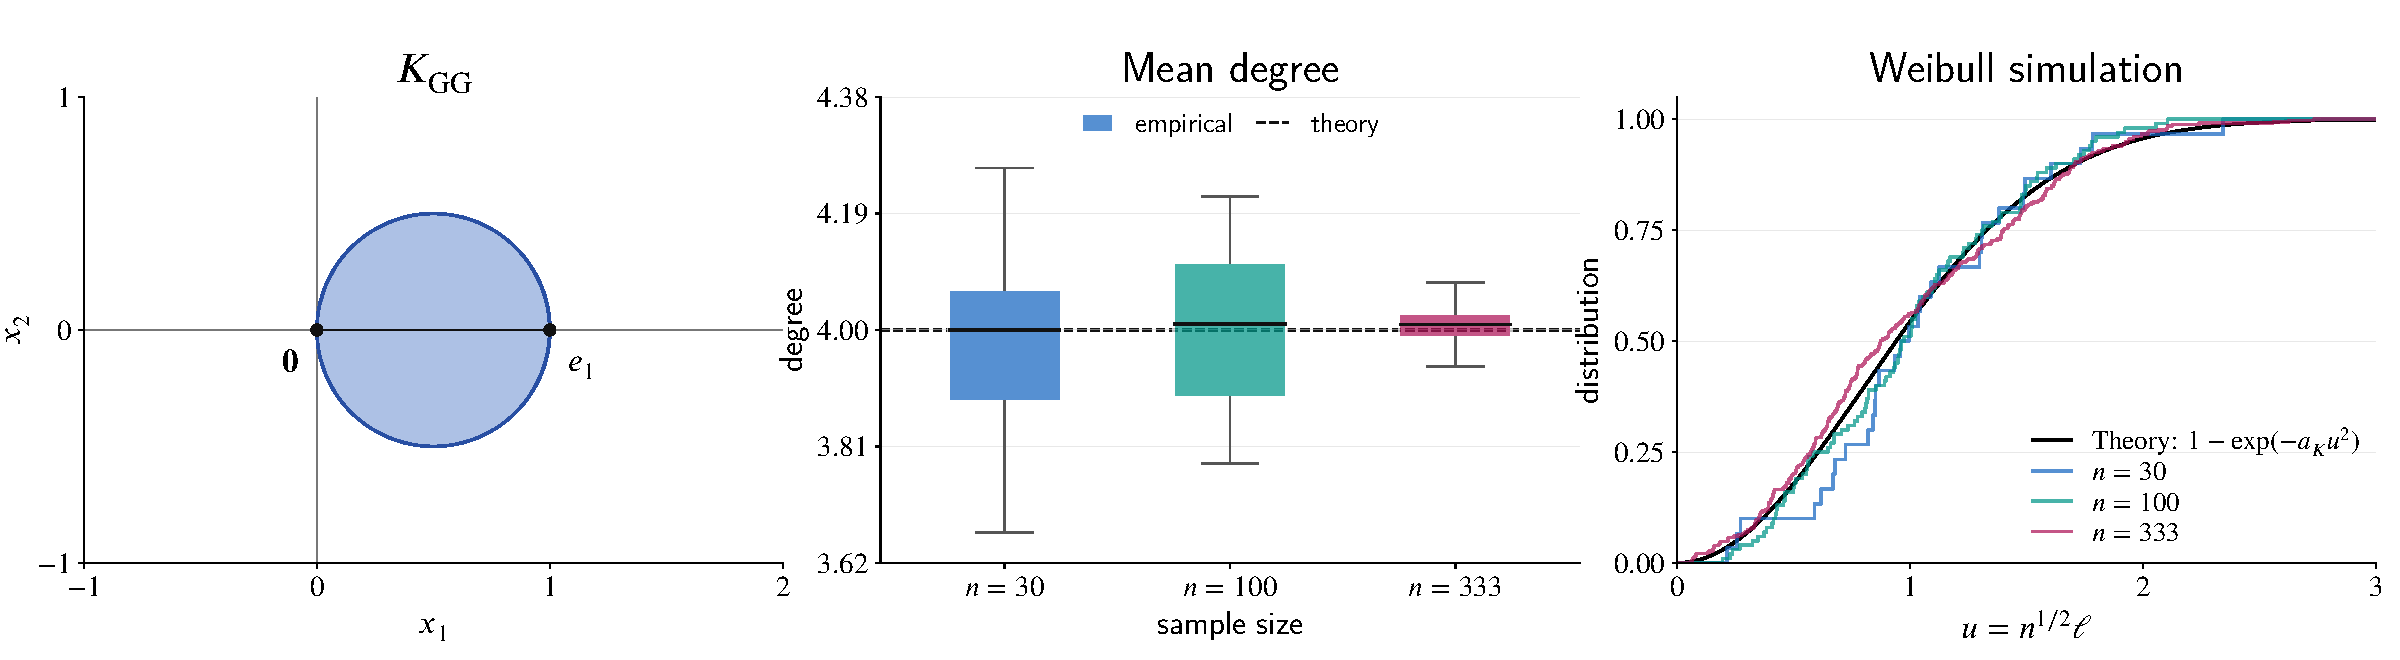
\includegraphics[width=\columnwidth]{fig_dashboard_r2_gg.pdf}
\caption{Numerical results for the planar Gabriel graph: unit region,
empirical mean degree, and rescaled edge-length distributions.}
\label{fig:gg-region}
\end{figure}

\begin{corollary}[Relative-neighborhood region]
\label{cor:rng-region-volume}
For
\begin{equation}\label{eq:rng-region-def}
K_{\mathrm{RNG}} = B(\0,1)\cap B(e_1,1),
\end{equation}
the unit region volume is
\begin{equation}\label{eq:rng-constant}
a_{d,\mathrm{RNG}} = \kappa_d I_{3/4} \left(\frac{d+1}{2},\frac{1}{2}\right).
\end{equation}
\end{corollary}

\begin{proof}
Apply Proposition~\ref{prop:two-ball-region-volume} with $\mathrm{r}_0=\mathrm{r}_1=1$ and $\delta=1$. The two caps have common height $1/2$.
\end{proof}

\begin{figure}[width=\columnwidth,pos=ht]
\centering
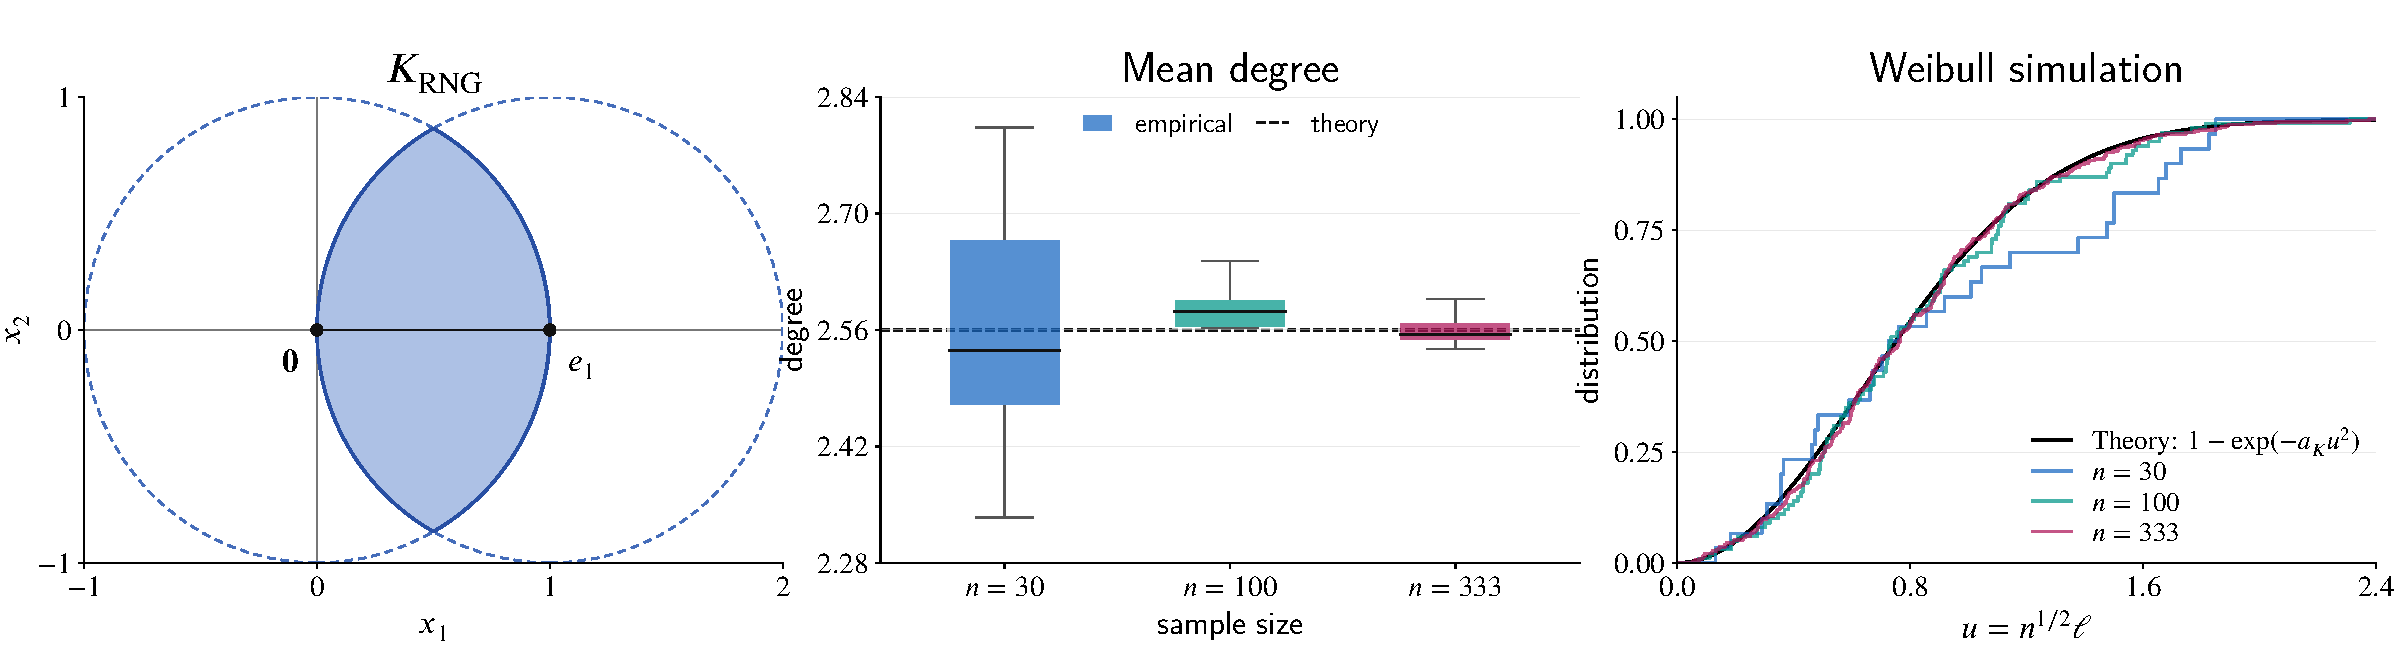
\includegraphics[width=\columnwidth]{fig_dashboard_r2_rng.pdf}
\caption{Numerical results for the planar relative-neighborhood graph:
unit region, empirical mean degree, and rescaled edge-length
distributions.}
\label{fig:rng-region}
\end{figure}

\begin{corollary}[Lune-based $\beta$-skeleton region]
\label{cor:beta-region-volume}
For $\beta \geq 1$, let
\begin{equation}\label{eq:beta-region-def}
K_{d,\beta} = B\left( \left(1-\frac{\beta}{2}\right)e_1, \frac{\beta}{2} \right) \cap B\left( \frac{\beta}{2}e_1, \frac{\beta}{2} \right).
\end{equation}
Then
\begin{equation}\label{eq:beta-volume-constant}
a_{d,\beta} = \kappa_d \left(\frac{\beta}{2}\right)^d I_{\frac{2\beta-1}{\beta^2}} \left(\frac{d+1}{2},\frac{1}{2}\right).
\end{equation}
\end{corollary}

\begin{proof}

The two balls have common radius $\beta/2$, center separation $\beta-1$, and cap height $1/2$. Proposition~\ref{prop:two-ball-region-volume} therefore gives the stated formula.
\end{proof}


\begin{figure}[width=\columnwidth,pos=ht]
\centering
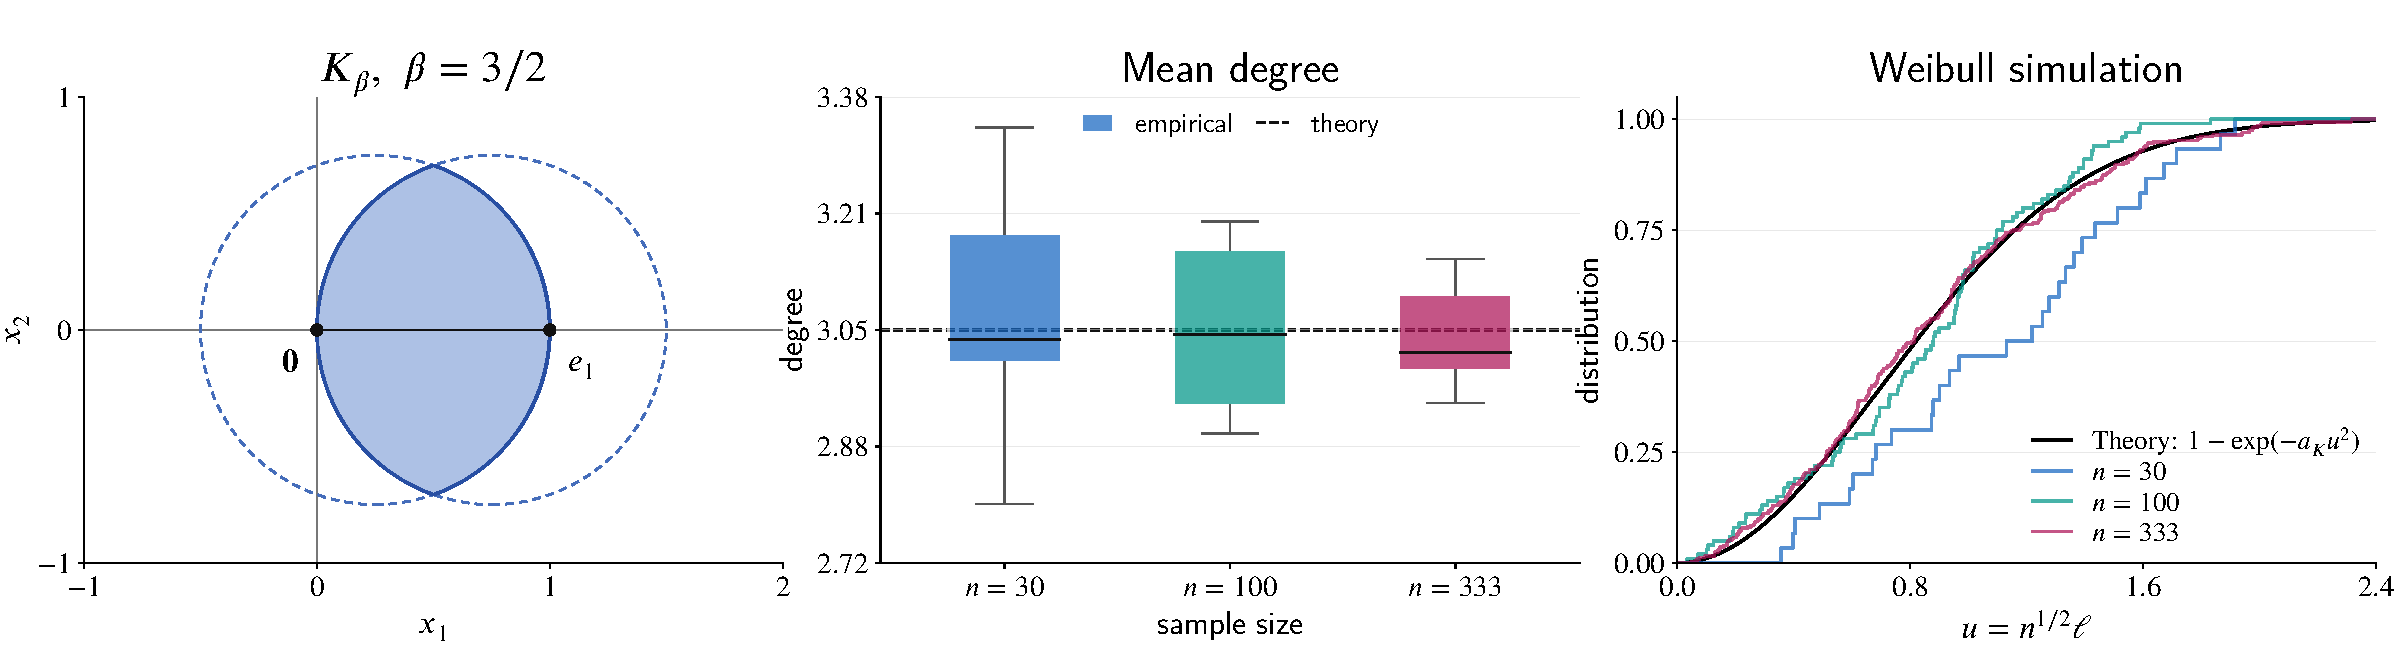
\includegraphics[width=\columnwidth]{fig_dashboard_r2_beta15.pdf}
\caption{Numerical results for the planar lune-based
\(\beta\)-skeleton with \(\beta=3/2\): unit region, empirical mean
degree, and rescaled edge-length distributions.}
\label{fig:beta_skeleton-region}
\end{figure}


\subsection{Stepping-stone diversion regions}

For $\alpha\ge 1$, define the stepping--stone region
\begin{equation}\label{eq:ss-region}
\begin{aligned}
S_{\mathrm{SS},\alpha}(p,q)
&=\bigl\{z\in\R^d:
  \norm{z-p}^{\alpha}\\
&\qquad{}+\norm{z-q}^{\alpha}
  \le \ellpq^{\alpha}\bigr\}.
\end{aligned}
\end{equation}
It has unit representative
\begin{equation}
        K_{\mathrm{SS},\alpha}
        =
        \set{z\in\R^d:
        \norm{z}^{\alpha}+\norm{z-e_1}^{\alpha}\le1}.
\end{equation}

For \(\alpha=1\), the triangle inequality forces the region to be
the segment \([p,q]\), which has zero \(d\)-dimensional volume.
Thus \(\alpha=1\) lies outside the positive-volume unit-region class
of Definition~3.1. For \(\alpha>1\), set
\begin{equation}\label{eq:ss-y-xprime}
\begin{aligned}
        y_\alpha(u)
        &=\frac12\left[
        4u^2-
        \left(1+u^2-(1-u^\alpha)^{\nicefrac{2}{\alpha}}\right)^2
        \right]^{\nicefrac12},\\
        x_\alpha'(u)
        &=u+u^{\alpha-1}
        \left(1-u^\alpha\right)^{\nicefrac{2-\alpha}{\alpha}}.
\end{aligned}
\end{equation}
Then
\begin{equation}\label{eq:ss-volume-constant}
        a_{d,\mathrm{SS}}(\alpha)
        =
        2\kappa_{d-1}
        \int_{2^{-\nicefrac{1}{\alpha}}}^1
        y_\alpha(u)^{d-1}x_\alpha'(u)\,\dd u.
\end{equation}


\noindent\emph{Proof.}
Normalize the pair \((p,q)\) to \((\0,e_1)\), parametrize one symmetric half of its boundary by \(u\), whose longitudinal coordinate has derivative \(x'_\alpha(u)\), and whose orthogonal \((d-1)\)-dimensional section is a ball of radius \(y_\alpha(u)\); integrating the section volume \(\kappa_{d-1}y_\alpha(u)^{d-1}\) with respect to \(x'_\alpha(u)\,du\), and doubling by symmetry, yields \eqref{eq:ss-volume-constant}.
\begin{figure}[width=\columnwidth,pos=ht]
\centering
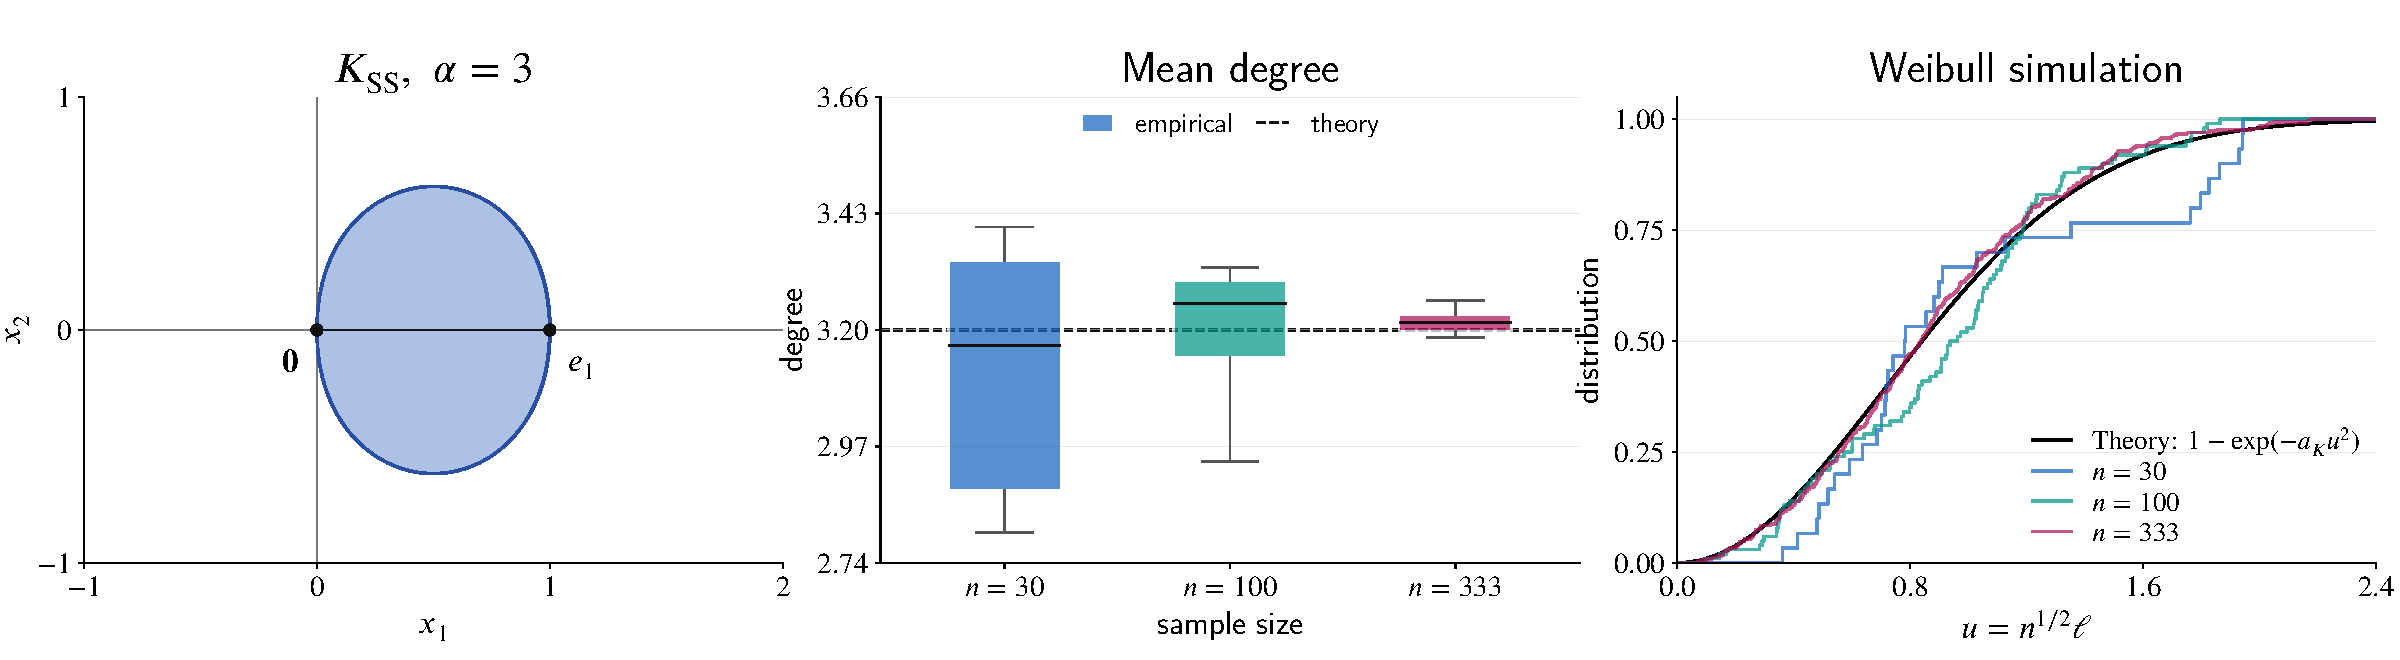
\includegraphics[width=\columnwidth]{fig_dashboard_r2_ss_alpha3.pdf}
\caption{Numerical results for the planar stepping--stone region with
\(\alpha=3\): unit region, empirical mean degree, and rescaled
edge-length distributions.}
\end{figure}


\subsection{Planar one-region Veltkamp subfamilies}
\label{sec:planar-veltkamp}
Lemma ~\ref{lem:li-cap-volume} applies directly to 
two planar one-region subfamilies of Veltkamp's
$\gamma$-neighborhood construction. Write
\begin{equation}
m := \frac{1}{2} e_1,
\qquad
e_2 := (0,1),
\end{equation}
and, for
\begin{equation}
    \gamma_0,\gamma_1\in(-1,1),
\qquad
|\gamma_0|\leq |\gamma_1|,
\end{equation}
define
\begin{equation}
\label{eq:veltkamp-one-region-radius-height}
R_\gamma
:=
\frac{1}{2(1-|\gamma|)},
\qquad
h_\gamma
:=
\frac{\sqrt{|\gamma|(2-|\gamma|)}}
{2(1-|\gamma|)}.
\end{equation}
For the nonsymmetric planar regions considered below, we use the
unique orientation-preserving rotation
\begin{equation}
R_{p,q}\in SO(2)
\end{equation}
satisfying
\begin{equation}
R_{p,q}e_1=u_{p,q}.
\end{equation}
This fixes the orientation of the normalized region relative to each
ordered pair \((p,q)\).

\paragraph{The \((0,\gamma)\)-subfamily.}
For \(\gamma_0=0\) and \(\gamma_1=\gamma\), set
\begin{equation}
D_0:=B\left(m,\frac12\right),
\qquad
D_\gamma:=B(m+h_\gamma e_2,R_\gamma).
\end{equation}
The construction has one prescribed neighborhood, namely
\begin{equation}
\label{eq:veltkamp-zero-region}
K_{0,\gamma}
:=
\begin{cases}
D_0\cap D_\gamma,
&
\gamma<0, \\[1mm]
D_0,
&
\gamma=0, \\[1mm]
D_0\cup D_\gamma,
&
\gamma>0.
\end{cases}
\end{equation}
Thus the \((0,\gamma)\)-subfamily is of intersection type for
\(\gamma<0\) and of union type for \(\gamma>0\). 

\begin{figure}[width=\columnwidth,pos=ht]
\centering
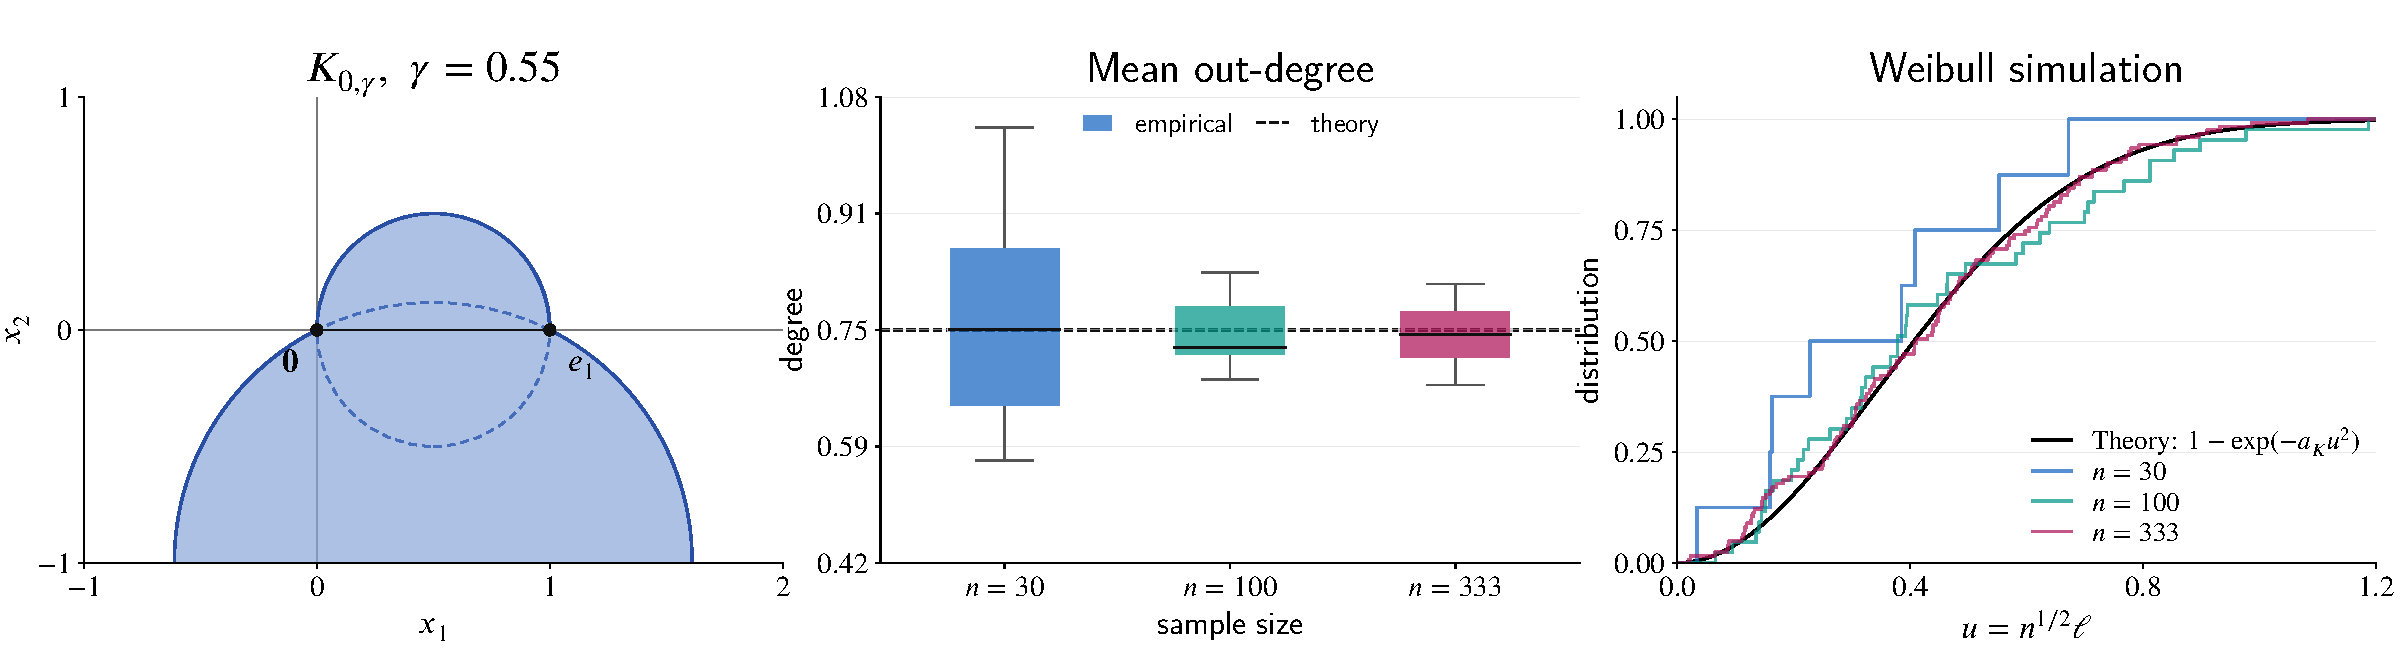
\includegraphics[width=\columnwidth]{fig_dashboard_r2_twoball_cup.pdf}
\caption{Numerical results for the planar \((0,\gamma)\)-subfamily with
\(\gamma=0.55\): unit region, empirical mean out-degree, and rescaled
edge-length distributions.}
\end{figure}

\paragraph{Diagonal $(\gamma,\gamma)$-subfamily.}
When
\begin{equation}
\gamma_0 = \gamma_1 = \gamma,
\end{equation}


For \(\gamma\in(-1,1)\setminus\{0\}\), write
\begin{equation}
D_\gamma^\pm
:=
B\!\left(m\pm h_\gamma e_2,R_\gamma\right).
\end{equation}

The original diagonal Veltkamp construction is recovered by coupling
the set operation to the sign of \(\gamma\):
\begin{equation}
\label{eq:diagonal-veltkamp-region}
K_{\gamma,\gamma}
:=
\begin{cases}
D_\gamma^{-}\cap D_\gamma^{+},
&
-1<\gamma<0,
\\[1mm]
B\left(m,\frac12\right),
&
\gamma=0,
\\[1mm]
D^-_\gamma \cup D^+_\gamma,
&
0<\gamma<1.
\end{cases}
\end{equation}

\begin{corollary}[Diagonal Veltkamp subfamily and the circle-based
\(\beta\)-skeleton]
For \(\gamma\in(-1,1)\), the planar diagonal Veltkamp subfamily
\(K_{\gamma,\gamma}\) coincides with the circle-based
\(\beta\)-skeleton in Veltkamp's normalized parameterization, with
\begin{equation}
\beta_{\mathrm{norm}}=\gamma.
\end{equation}
Equivalently, if \(\beta>0\) denotes the standard nonnegative
circle-based parameter, then
\begin{equation}
\beta=
\begin{cases}
1+\gamma,
&
-1<\gamma\leq 0,
\\[1mm]
\dfrac{1}{1-\gamma},
&
0\leq\gamma<1.
\end{cases}
\end{equation}
\end{corollary}

\begin{proof}
For \(\gamma<0\), the circle-based neighborhood is the intersection
of two disks of radius
\begin{equation}
\frac{1}{2(1+\gamma)}
=
\frac{1}{2(1-|\gamma|)}
=
R_\gamma.
\end{equation}
For \(\gamma>0\), it is the union of two disks of radius
\begin{equation}
\frac{\beta}{2}
=
\frac{1}{2(1-\gamma)}
=
R_\gamma.
\end{equation}
At \(\gamma=0\), both constructions reduce to the Gabriel disk.
\end{proof}


\begin{figure}[width=\columnwidth,pos=ht]
\centering
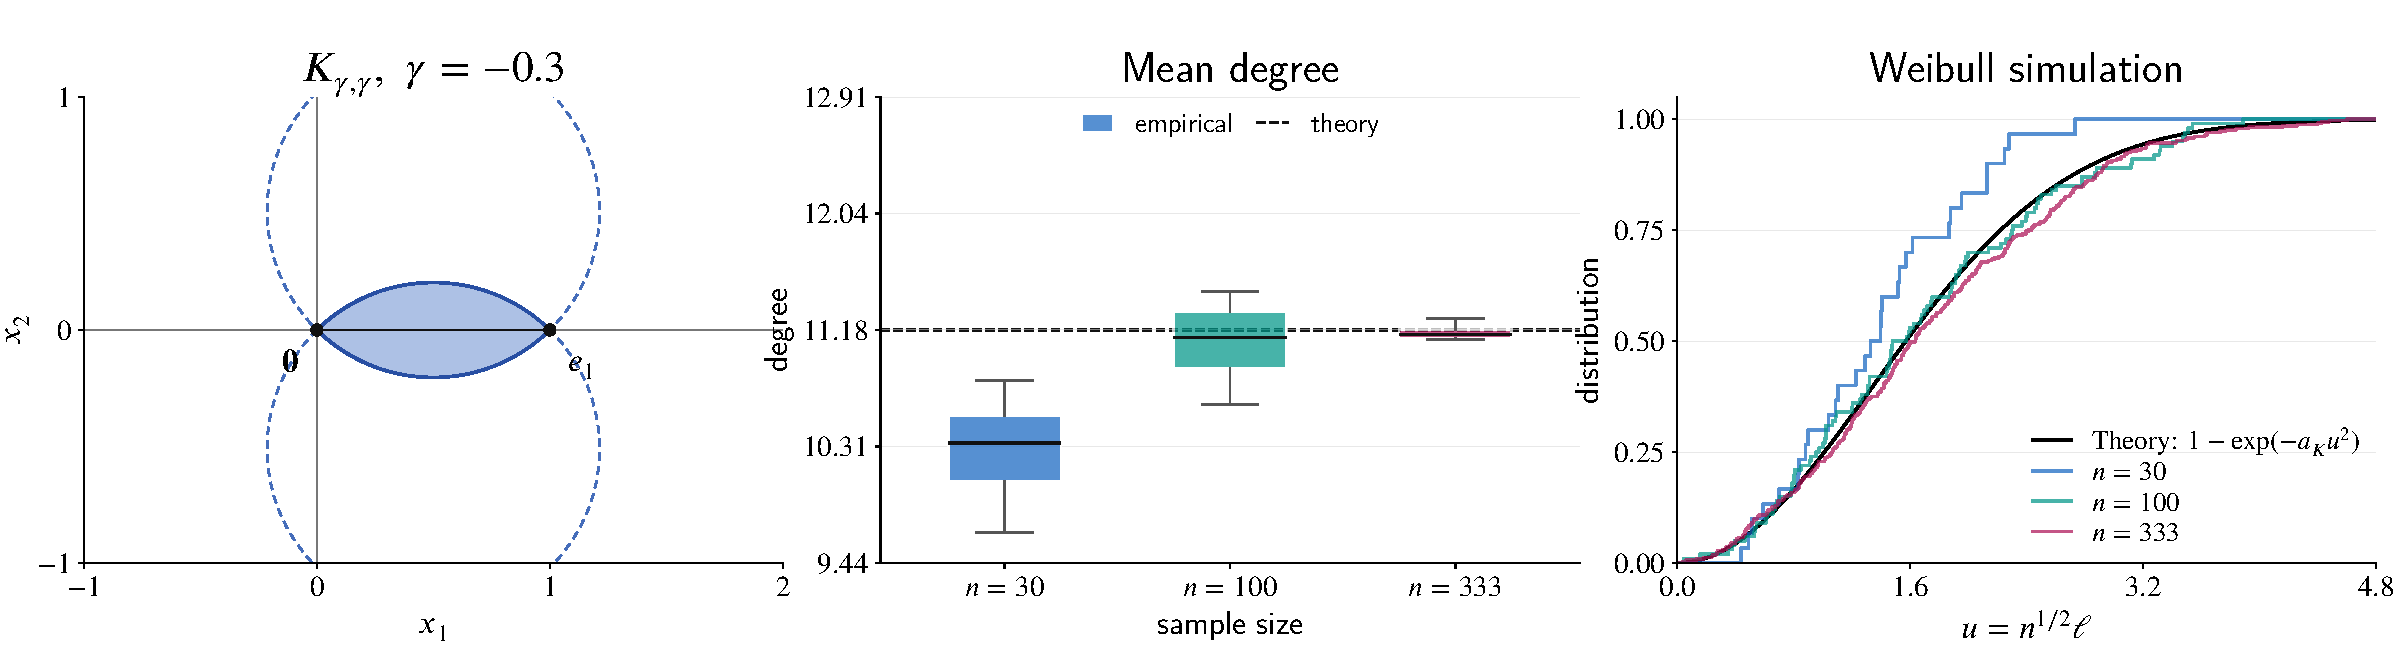
\includegraphics[width=\columnwidth]{fig_dashboard_r2_twoball_cap_gamma03.pdf}
\caption{Numerical results for the planar diagonal
\((\gamma,\gamma)\)-subfamily with \(\gamma=-0.3\): unit region,
empirical mean degree, and rescaled edge-length distributions.}
\end{figure}


These two subfamilies are full prescribed empty-region graphs. For
general parameter pairs $(\gamma_0,\gamma_1)$, Veltkamp's
construction may involve two alternative neighborhoods and is not, in
general, determined by the emptiness of one prescribed pair region.








\paragraph{\(\gamma\)-parameterized planar regions.}
\label{sec:gamma-two-ball-regions}
Set
\begin{equation}
\label{eq:gamma-two-ball-epsilon}
\epsilon_{\gamma_0,\gamma_1}
:=
\begin{cases}
-1,
&
\gamma_0\gamma_1>0,
\\[1mm]
1,
&
\gamma_0\gamma_1\leq0.
\end{cases}
\end{equation}
Define the two disks
\begin{equation}
\label{eq:gamma-two-ball-disks}
\begin{aligned}
D_{\gamma_0,\gamma_1}^{(0)}
&:=B\left(
\begin{gathered}
m+h_{\gamma_0}e_2,
\\[-1mm]
R_{\gamma_0}
\end{gathered}
\right),\\
D_{\gamma_0,\gamma_1}^{(1)}
&:=B\left(
\begin{gathered}
m+\epsilon_{\gamma_0,\gamma_1}h_{\gamma_1}e_2,
\\[-1mm]
R_{\gamma_1}
\end{gathered}
\right).
\end{aligned}
\end{equation}
The \(\gamma\)-parameterized two-ball region is
\begin{equation}
\label{eq:gamma-two-ball-region}
K_{\gamma_0^-,\gamma_1^-}
:=
\begin{cases}
D_{\gamma_0,\gamma_1}^{(0)}
\cap
D_{\gamma_0,\gamma_1}^{(1)},
&
\gamma_1<0,
\\[1mm]
B\left(m,\frac12\right),
&
\gamma_0=\gamma_1=0,
\\[1mm]
D_{\gamma_0,\gamma_1}^{(0)}
\cup
D_{\gamma_0,\gamma_1}^{(1)},
&
\gamma_1>0.
\end{cases}
\end{equation}

This parameterization is useful because it selects one prescribed pair
region \(S(p,q)\) for each candidate pair, rather than requiring the
two alternative neighborhoods that may arise in Veltkamp's general
planar construction. Consequently, the selected rule belongs to the
unit-region framework, so the factorization, Poisson void, mean
out-degree, and incident-edge length identities derived above apply
directly.


\begin{figure}[width=\columnwidth,pos=ht]
\centering
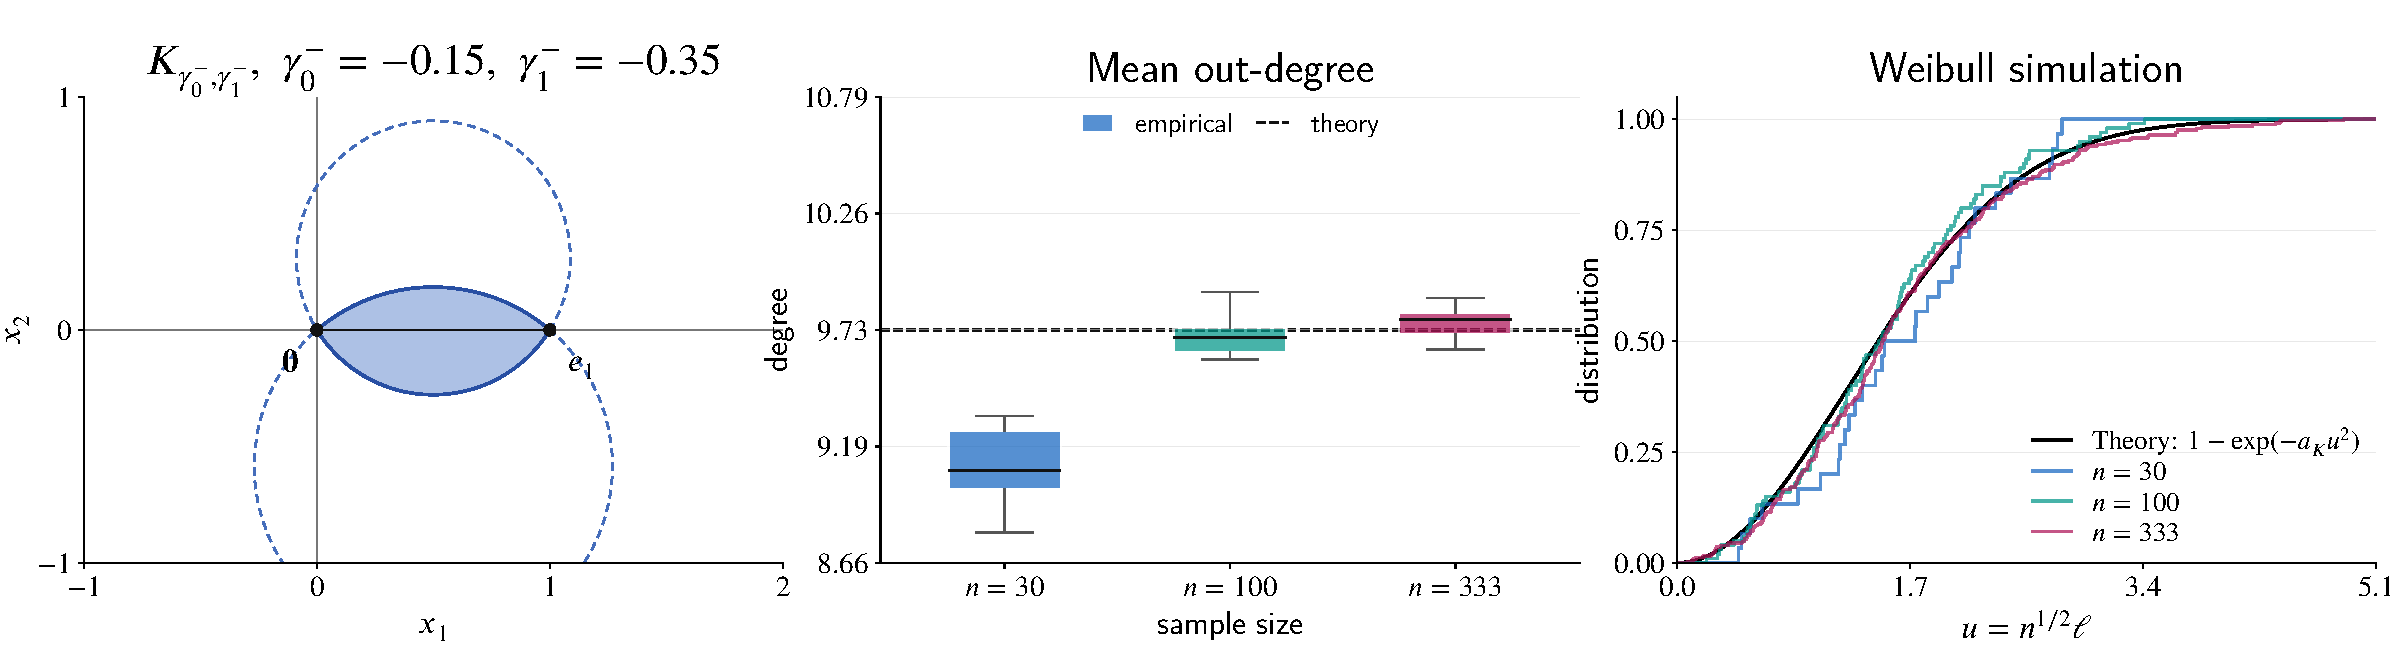
\includegraphics[width=\columnwidth]{fig_dashboard_r2_twoball_cap.pdf}
\caption{Numerical results for the planar \(\gamma\)-parameterized
two-ball region with \(\gamma_0=-0.15\) and \(\gamma_1=-0.35\):
unit region, empirical mean out-degree, and rescaled edge-length
distributions.}
\end{figure}

\subsection{Densities}

For a fixed ambient dimension \(d\) and a fixed Poisson intensity
\(\rho\), the normalized Palm edge-length law depends on the
particular unit region \(K\) only through its volume \(a_K\). Indeed,
\begin{equation}
g_K(\ell)
=
\rho d a_K \ell^{d-1}
\exp\left\{-\rho a_K\ell^d\right\},
\qquad
\ell\geq0.
\end{equation}
Thus, when \(d\) and \(\rho\) are held fixed, the Weibull shape
parameter remains unchanged, whereas the unit-region volume \(a_K\)
is the only rule-specific quantity affecting the scale parameter
\((\rho a_K)^{-1/d}\). In particular, regions with larger volume
produce shorter characteristic edge lengths.

\begin{figure}[width=\columnwidth,pos=ht]
\centering
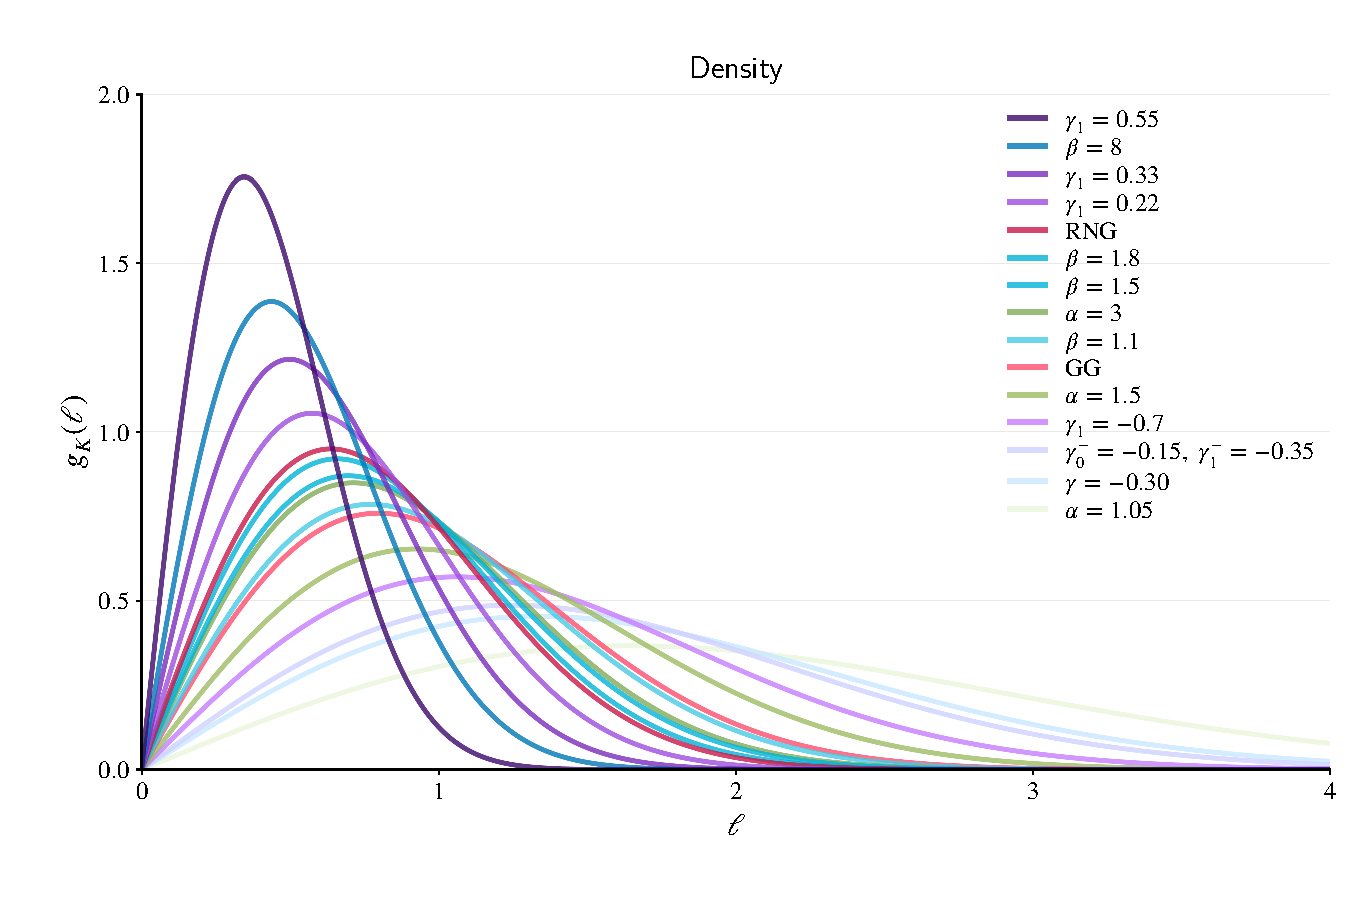
\includegraphics[width=\columnwidth]{fig_r2_weibull_all_density.pdf}
\caption{Theoretical planar edge-length densities for the normalized
regions at unit intensity. Larger unit-region areas shift the densities
toward shorter edge lengths; the curves correspond to the graph families
described above.}
\end{figure}



\section{Discussion}\label{sec:discussion}

\subsection{Region volume as a geometric complexity parameter}
A key feature of the present framework is that, for finite similarity-region empty-region rules, the volume of the unit region,
\begin{equation}\label{eq:normalized-region-volume-def}
a_K = \lambda_d(K),
\end{equation}
acts as a geometric complexity parameter. The factorization
\begin{equation}\label{eq:factorization-volume-metric}
\lambda_d(S(p,q)) = a_K\|p-q\|^d
\end{equation}
shows that the effect of the exclusion rule on the volume of the
region associated with a pair is completely captured by \(a_K\).
Consequently, at the fixed-pair and first-moment levels, proximity
rules with different shapes but the same unit-region volume have the
same Poisson void probability as a function of pair length, the same
mean out-degree of a typical point, and the same normalized
incident-edge length law. For symmetric rules, the out-degree
coincides with the ordinary degree.

This interpretation gives \(a_K\) a direct geometric and probabilistic
meaning. A larger value of \(a_K\) corresponds to a more restrictive
exclusion rule: the region that must be empty for a pair to form an
edge is larger, so edges occur less frequently. Quantitatively, the
mean out-degree of a typical point is \(\kappa_d/a_K\). For symmetric
rules, this is also the mean degree. The characteristic incident-edge
length scale is \((\rho a_K)^{-\nicefrac{1}{d}}\). Thus the region
volume simultaneously controls graph sparsity and the scale of the
edges that remain.



\subsection{Explicit families and computable consequences}
The formulas for lune-based $\beta$-skeleton regions, selected planar two-ball regions associated with Veltkamp's construction, and stepping--stone diversion regions demonstrate that the general factorization is not merely formal. For these families, explicit or one-dimensional integral expressions for the unit region volume make it possible to obtain concrete edge probabilities, mean out-degrees, and, for symmetric subfamilies, mean degrees,
together with Weibull scales.

This separation is useful because the same stochastic formulas apply to every admissible region, whereas the geometric calculation of $a_K$ depends on the particular rule. Ball-generated regions can be treated through hyperspherical-cap formulas, while the stepping--stone family leads naturally to a different integral representation. The framework therefore accommodates distinct geometric mechanisms without requiring a new probabilistic derivation for each graph family.





\subsection{Scope and limitations of the pairwise-region framework}
\paragraph{Constructions beyond prescribed pairwise regions.}

The framework requires one prescribed finite region $S(p,q)$ for each candidate pair. Delaunay adjacency is existential: two points are joined by an edge when some sphere with the two points on its boundary and center on their perpendicular-bisector hyperplane is empty \citep{devroye1988expected}; thus the test ranges over a family of balls rather than one prescribed region $S(p,q)$.

Veltkamp's $\gamma$-neighborhood construction requires a separate qualification. In ambient dimension $d \geq 3$, its defining neighborhood is associated with $d$ sites $(x_1, \ldots, x_d)$, and an empty neighborhood joins all $\binom{d}{2}$ pairs among those sites. It is therefore a higher-arity construction rather than a prescribed pairwise rule.

Voronoi cells are determined by comparisons with all sites, whereas the Euclidean minimum spanning tree is selected by a global optimization criterion. These constructions are closely related to the present graphs, but do not fall within the prescribed finite pairwise-region framework without additional analysis \citep{devroye1988expected,toussaint1980relative,jaromczyk1992relative,veltkamp1992gamma,penrose2001central}.

\paragraph{Infinite-volume regions.}
Infinite strips and halfspaces may be similarity-covariant, but they satisfy
\begin{equation}\label{eq:infinite-region-volume-limit}
\lambda_d(K) = \infty.
\end{equation}
For example, in the lune-based $\beta$-skeleton family, the limiting region as $\beta \to \infty$ is the infinite slab bounded by the hyperplanes through $p$ and $q$ perpendicular to $q-p$; in the plane, this is the usual infinite strip \citep{cardinal2009empty}. Consequently, the finite-volume Poisson void formulas and the constants derived here do not apply directly \citep{devroye1988expected,veltkamp1992gamma}.


\subsection{Limits of the first-moment theory}
The reduction to $a_K$ has a precise scope. It governs one-pair void probabilities and Palm first-moment quantities, but it does not determine joint statistics of distinct edges. For example, degree variances, edge-length correlations, and factorial moment measures depend on the overlap geometry of two or more exclusion regions. These quantities involve volumes such as
\begin{equation}\label{eq:exclusion-region-overlap}
\lambda_d\bigl(S(0,x)\cup S(0,y)\bigr),
\end{equation}
which cannot generally be recovered from the single scalar $a_K$.

The framework is also restricted to prescribed finite pairwise regions. Delaunay adjacency, Voronoi constructions, Euclidean minimum spanning trees, infinite-volume regions, and cone constructions based on an external orientation convention fall outside this setting for different structural reasons. These exclusions are not defects of the factorization theorem; rather, they identify which geometric mechanisms must be incorporated by a more general theory.

\subsection{Directions beyond Euclidean similarity regions}
A natural extension is to normed or anisotropic settings. In Euclidean space, rotation covariance makes the volume constant independent of the direction of the pair.
Let \(\|\cdot\|_L\) denote a norm on \(\mathbb{R}^d\) with unit ball
\(L\).
In a general normed space or under anisotropic pairwise rules, the exclusion-region volume may instead take the form
\begin{equation}\label{eq:anisotropic-volume-direction}
\lambda_d(S(p,q)) = a(u)\norm{p-q}_L^d,
\end{equation}
where $u$ denotes the direction of $q-p$. In that setting, conditional edge-length laws may remain Weibull in each direction, while the unconditional law becomes a directional mixture. Characterizing the rules for which a direction-independent Weibull law persists would extend the present universality result.

A second direction is higher-order Palm analysis. Explicit formulas for degree variance, joint incident-edge statistics, and stabilization properties would require a systematic treatment of exclusion-region overlaps. 

Finally, the exact Weibull law suggests statistical questions. It would be natural to investigate how the effective scale \(\rho a_K\) can be estimated or tested from observed proximity graphs, and whether departures from the predicted law can be used to diagnose anisotropy, spatial inhomogeneity, or non-Poisson interaction.


\section{Conclusion}\label{sec:conclusion}
Finite similarity-region empty-region rules admit a simple geometric
reduction: their pairwise region volumes are determined by the unit
region volume \(a_K\). This reduction yields exact Poisson void
probabilities, first-moment directed-edge statistics, and a Weibull law
for incident-edge lengths. For symmetric rules, these directed-edge
results yield the corresponding undirected degree and typical-edge
statements. Explicit constants
for ball-generated and stepping--stone regions show that the theory
applies to several classical and nonclassical proximity constructions.
The remaining challenge is to move beyond one-pair and first-moment quantities
toward overlap-sensitive, anisotropic, and higher-order theories.



\section*{Data availability}

No external datasets were used or analyzed in this study. The numerical
results were obtained from point-process simulations generated
using the \texttt{ProximityGraphs} Python package \citep{proximitygraphs}.

\section*{Declaration of competing interest}
The authors declare no competing interests.

\section*{Declaration of generative AI and AI-assisted technologies in the manuscript preparation process}
During the preparation of this work, the authors used ChatGPT, an AI language model by OpenAI, to assist with drafting descriptions of figures and tables and with improving language, clarity, and structure. After using this tool, the authors reviewed and edited the content as needed and take full responsibility for the content of the published article. No generative AI tool was used to generate research data, conduct simulations, or replace the mathematical derivations and verification reported in the manuscript.

\section*{Funding}
This research did not receive any specific grant from funding agencies in the public, commercial, or not-for-profit sectors.


\printcredits

\bibliographystyle{cas-model2-names}
\bibliography{references}


\clearpage
\onecolumn
\appendix

\section{Applied uses of fixed-region proximity graphs}

The same empty-region regions also appear outside the Poisson setting.  In
these applications the point set is usually observed, constructed, or simulated,
and the graph is used as a geometric summary of adjacency, obstruction, or
movement.  Table~\ref{tab:applications} records the role of the region in each setting; it is
not an extension of the Poisson formulas above.

\begin{table}[width=.82\linewidth,cols=3,pos=ht]
\caption{Applied settings where fixed-region proximity graphs are used as geometric adjacency rules.}\label{tab:applications}
\small
\renewcommand{\arraystretch}{1.35}
\setlength{\tabcolsep}{3.5pt}
\begin{tabular*}{\tblwidth}{@{\extracolsep{\fill}}
  >{\RaggedRight\arraybackslash}p{0.15\FullWidth}
  >{\RaggedRight\arraybackslash}p{0.19\FullWidth}
  >{\RaggedRight\arraybackslash}p{0.43\FullWidth}
  @{}}
\toprule
Source & Setting & Role of the region \\
\midrule
\citep{gabriel1969statistical,matula1980gabriel} &
{Geographic variation and clustering} &
The Gabriel disk with diameter $pq$ is used as a local adjacency criterion for geographic data analysis. \\
\vspace{2pt} \\
\citep{toussaint1980relative,jaromczyk1992relative} &
{Computational morphology and spatial analysis} &
Gabriel, relative-neighborhood, and $\beta$-skeleton regions encode neighborhood and shape information in finite planar point sets. \\
\vspace{2pt} \\
\citep{watanabe2008evaluating} &
{Transportation-network models} &
Proximity graphs are compared as idealized road-network skeletons and evaluated through travel-efficiency criteria. \\
\vspace{2pt} \\
\citep{maravillo2023recovering,maravillo2024modelacion} &
{Street-network and tiling models} &
$\beta$-skeleton regions are used to recover cyclic tiling graphs motivated by empirical street-network structures. \\
\vspace{2pt} \\
\citep{kannangara2018stepping} &
{Public movement analysis} &
The stepping--stone region gives a parameterized diversion corridor bounded between the Gabriel case and the relative-neighborhood case. \\
\vspace{2pt} \\
\citep{jurkiewicz2023topohub} &
Network topology generation &
Gabriel graph regions are used to generate reproducible reference physical network topologies in structural design. \\
\bottomrule
\end{tabular*}
\end{table}



\clearpage
\section{Consequences of the unit-volume constant (\(a_K\))}
\begin{table}[width=.78\linewidth,cols=3,pos=ht]
\caption{Poisson--Palm and Weibull consequences of the unit-volume constant (\(a_K\)).}\label{tab:poisson-palm-weibull-summary}
\small
\renewcommand{\arraystretch}{1.35}
\setlength{\tabcolsep}{3.5pt}
\begin{tabular*}{\tblwidth}{@{\extracolsep{\fill}}
  >{\RaggedRight\arraybackslash}p{0.10\FullWidth}
  >{\RaggedRight\arraybackslash}p{0.16\FullWidth}
  >{\RaggedRight\arraybackslash}p{0.48\FullWidth}
  @{}}
\toprule
Source & Result & Exact consequence \\
\midrule

Cor.~\ref{cor:fixed-pair} & 
{Fixed-pair void law} & 
$\displaystyle \Pp\left\{ \Phi\bigl(S(p,q) \setminus \{p,q\}\bigr)=0 \right\} = \exp\left\{-\rho a_K \ellpq^d\right\}$ \\
\vspace{2pt} \\

Cor.~\ref{cor:typical-pair} & 
{Typical points void law} & 
$\displaystyle \Pp^{p,q}\left\{ \Phi^{!}_{p,q}\bigl(S(p,q)\bigr)=0 \right\} = \exp\left\{-\rho a_K \ellpq^{d}\right\}$ \\
\vspace{2pt} \\

Cor.~\ref{cor:palm-mecke} & 
{Palm--Mecke identity} & 
$\displaystyle \E^{\0}\left[ \sum_{x\in\Phi_\0^!} g(x)\chi_K(x;\Phi_\0^!) \right] = \rho\int_{\R^d} g(x) \exp\left\{-\rho a_K\ellox^{d}\right\} \,\dd x$ \\
\vspace{2pt} \\

Def.~\ref{def:palm-length-measure} & 
{Incident-edge length measure} & 
$\displaystyle \nu_K(C) = \E^{\0}\left[ \sum_{x\in\Phi_\0^!} \chi_K(x;\Phi_\0^!) \1\left\{\ellox\in C\right\} \right]$ \\
\vspace{2pt} \\

Cor.~\ref{cor:palm-intensity} & 
{Incident-edge length density} & 
$\displaystyle \nu_K(\dd r) = \rho d \kappa_d r^{d-1} \exp\left\{-\rho a_K r^d\right\} \,\dd r$ \\
\vspace{2pt} \\

Cor.~\ref{cor:mean-outdegree} & 
{Mean out-degree} & 
$\displaystyle \E^{z}\left[\deg_{\mathrm{out}}(z)\right] = \frac{\kappa_d}{a_K}, \qquad z \in \R^d$ \\
\vspace{2pt} \\

Cor.~\ref{cor:edge-intensity-per-vertex} & 
{Undirected edge intensity} & 
$\displaystyle \frac{\rho_{E,K}}{\rho} = \frac{\kappa_d}{2a_K} \quad \text{(for symmetric rules)}$ \\
\vspace{2pt} \\

Def.~\ref{def:palm-edge-length-distribution} & 
{Palm edge distribution} & 
$\displaystyle \mu_K(C) = \frac{\nu_K(C)}{\nu_K([0,\infty))}, \qquad L_K \sim \mu_K$ \\
\vspace{2pt} \\

Thm.~\ref{thm:palm-edge-length-weibull} & 
{Weibull law} & 
$\displaystyle L_K \sim \operatorname{Weibull}\left( d, \, (\rho a_K)^{-\nicefrac{1}{d}} \right)$ \\
\vspace{2pt} \\

Cor.~\ref{cor:universal-palm-edge-scaling} & 
{Universal scaling} & 
$\displaystyle Z_K := (\rho a_K)^{\nicefrac{1}{d}} L_K \sim \operatorname{Weibull}(d,1)$ \\
\vspace{2pt} \\

Cor.~\ref{cor:universal-palm-edge-scaling} & 
{Exponential transform} & 
$\displaystyle U_K := \rho a_K L_K^d \sim \operatorname{Exp}(1)$ \\

\bottomrule
\end{tabular*}
\begin{minipage}{\tblwidth}
\vspace{5pt}
\scriptsize Here \(a_K=\lambda_d(K)\), and
\(\chi_K(x;\eta)\) is the indicator that the pair region
\(S(\0,x)\) contains no point of \(\eta\) other than its
endpoints.
\end{minipage}
\end{table}


\clearpage
\section{First-order distributional characteristics of edge length}
\label{app:weibull-consequences}

\begin{table}[width=.78\linewidth,cols=2,pos=ht]
\caption{Derived distributional characteristics of the length \(L_K\) of a typical incident edge}
\label{tab:weibull-derived-consequences}
\small
\renewcommand{\arraystretch}{1.35}
\setlength{\tabcolsep}{3.5pt}
\begin{tabular*}{\tblwidth}{@{\extracolsep{\fill}}
  >{\RaggedRight\arraybackslash}p{0.30\FullWidth}
  >{\RaggedRight\arraybackslash}p{0.42\FullWidth}
  @{}}
\toprule
Quantity & Formula \\
\midrule

% --- Section 1: Fundamental Distribution Functions ---
Length distribution &
$\displaystyle L_K \sim \operatorname{Weibull} \left(d, (\rho a_K)^{-\nicefrac{1}{d}} \right)$ \\
\vspace{2pt} \\

Distribution function &
$\displaystyle \Pp\{L_K\le \ell\} = 1-\exp\{-\rho a_K\ell^d\}, \qquad \ell\ge0$ \\
\vspace{2pt} \\

Density &
$\displaystyle g_K(\ell) = d\rho a_K\ell^{d-1} \exp\{-\rho a_K\ell^d\}, \qquad \ell\ge0$ \\
\vspace{2pt} \\

Hazard function &
$\displaystyle h_K(\ell) = d\rho a_K\ell^{d-1}, \qquad \ell > 0$ \\
\vspace{2pt} \\

Cumulative hazard function &
$\displaystyle H_K(\ell) = \rho a_K\ell^d, \qquad \ell\ge0$ \\
\vspace{2pt} \\

% --- Section 2: Quantiles and Partitioning ---
\(p\)-quantile, \(0<p<1\) &
$\displaystyle Q(p) = (\rho a_K)^{-\nicefrac{1}{d}}[-\log(1-p)]^{\nicefrac{1}{d}}$ \\
\vspace{2pt} \\

Median &
$\displaystyle \operatorname{med}(L_K) = (\rho a_K)^{-\nicefrac{1}{d}}(\log 2)^{\nicefrac{1}{d}}$ \\
\vspace{2pt} \\

% --- Section 3: Moments and Dispersion ---
Raw moment &
$\displaystyle \mathbb{E}\!\left[L_K^m\right]
=
(\rho a_K)^{-m/d}
\Gamma\!\left(1+\frac{m}{d}\right),
\qquad m\geq 0$ \\
\vspace{2pt} \\

Mean length &
$\displaystyle \E[L_K] = (\rho a_K)^{-\nicefrac{1}{d}} \Gamma\left(1+\frac{1}{d}\right)$ \\
\vspace{2pt} \\

Variance &
$\displaystyle \operatorname{var}(L_K) = (\rho a_K)^{-\nicefrac{2}{d}} \left[ \Gamma\left(1+\frac{2}{d}\right) - \Gamma\left(1+\frac{1}{d}\right)^2 \right]$ \\
\vspace{2pt} \\

Coefficient of variation &
$\displaystyle \operatorname{CV}(L_K) = \left[ \frac{ \Gamma\left(1+\frac{2}{d}\right) }{ \Gamma\left(1+\frac{1}{d}\right)^2 } -1 \right]^{\nicefrac{1}{2}}$ \\
\vspace{2pt} \\

% --- Section 4: Transforms and Specializations ---
Exponential transform &
$\displaystyle \rho a_K(L_K)^d \sim \operatorname{Exp}(1)$ \\
\vspace{2pt} \\

Standardized edge length &
$\displaystyle (\rho a_K)^{\nicefrac{1}{d}}L_K \sim \operatorname{Weibull}(d,1)$ \\
\vspace{2pt} \\

Planar specialization, \(d=2\) &
$\displaystyle L_K \sim \operatorname{Rayleigh} \left( \frac{1}{\sqrt{2\rho a_K}} \right)$ \\

\bottomrule
\end{tabular*}

\begin{minipage}{\tblwidth}
\vspace{5pt}
\scriptsize
\end{minipage}
\end{table}


% \twocolumn





\end{document}
